\documentclass[12pt,a4paper]{report}


\usepackage{amsmath}
\usepackage[utf8]{inputenc}
\usepackage{amsmath}
\usepackage{amsfonts}
\usepackage{amssymb}
\usepackage{calrsfs}
\usepackage[left=2cm,right=2cm,top=2cm,bottom=2cm]{geometry}
\usepackage[mathscr]{euscript}

%%%%%For writing large opertors%%%%%%%%%%%
%\usepackage{stmaryrd}
%%%%%%%%%%%%%%%%%%%%%%%%%%%%%%%%%%%%%%%%%%

%%%%%%%%%%for writing large parallel%%%%%%
\usepackage{mathtools}
\DeclarePairedDelimiter\bignorm{\lVert}{\rVert}
%%%%%%%%%%%%%%%%%%%%%%%%%%%%%%%%%%%%%%%%%%

%%%for drawing commutative diagrams.%%%%%%
\usepackage{tikz-cd}  
%%%%%%%%%%%%%%%%%%%%%%%%%%%%%%%%%%%%%%%%%%

%%%%%%%%%%for changing margin
\def\changemargin#1#2{\list{}{\rightmargin#2\leftmargin#1}\item[]}
\let\endchangemargin=\endlist 

\newenvironment{proof}
{\begin{changemargin}{1cm}{0.5cm} 
	}%your text here
	{\end{changemargin}
}

\newenvironment{subproof}
{\begin{changemargin}{0.5cm}{0.5cm} 
	}%your text here
	{\end{changemargin}
}
%%%%%%%%%%%%%%%%%%%%%%%%%%%%%

\begin{document}
\newcommand{\thm}{\textbf{Theorem) }}
\newcommand{\thmnum}[1]{\textbf{Theorem #1) }}
\newcommand{\defi}{\textbf{Definition) }}
\newcommand{\definum}[1]{\textbf{Definition #1) }}
\newcommand{\lem}{\textbf{Lemma) }}
\newcommand{\lemnum}[1]{\textbf{Lemma #1) }}
\newcommand{\prop}{\textbf{Proposition) }}
\newcommand{\propnum}[1]{\textbf{Proposition #1) }}
\newcommand{\corr}{\textbf{Corollary) }}
\newcommand{\corrnum}[1]{\textbf{Corollary #1) }}
\newcommand{\pf}{\textbf{proof) }}

\newcommand{\lap}{\triangle} %%Laplacian
\newcommand{\s}{\vspace{10pt}}
\newcommand{\bull}{$\bullet$}
\newcommand{\sta}{$\star$}
\newcommand{\reals}{\mathbb{R}}

\newcommand{\eop}{\hfill  \textsl{(End of proof)} $\square$} %end of proof
\newcommand{\eos}{\hfill  \textsl{(End of statement)} $\square$} %end of proof


\newcommand{\intN}{\mathbb{Z}_N}
\newcommand{\nat}{\mathbb{N}}
\newcommand{\norms}[2]{\bignorm[\big]{#1}_{#2}}
\newcommand{\abs}[1]{\big| #1 \big|}
\newcommand{\avg}{\mathbb{E}}
\newcommand{\prob}{\mathbb{P}}
\newcommand{\borel}{\mathscr{B}}
\newcommand{\EE}{\mathscr{E}}
\newcommand{\pa}{\partial}

\renewcommand{\bar}{\overline}

\def\doubleunderline#1{\underline{\underline{#1}}}

\newcommand{\newday}{===============================================================}
\newcommand{\digression}{**********************************************************************************************}


\setlength\parindent{0pt}

\chapter*{Analysis of PDEs}
\s

Claude Warnick(cmw50)

www.dpmms.cam.ac.uk/$\sim$cmw50

Example Classes : Dr. Ivan Moyano
\s

Texts : (1)Evans. PDEs, (2)Rauch, PDEs, (3)F.John, PDEs, (4)Gilberg + Raudinger, Elliptic PDE, (5) Ladyzhenskay, The Boundary Value Problems of Mathematical Physics.
\s

\newday

(5th October 2018, Friday)
\s

\section*{Introduction}

Suppose $U \subset \reals^n$ is open. A \emph{partial differential equation} of order $k$ is an expression of the following form:
\begin{align}
F(x, u(x),Du(x),\cdots,D^{(k)}u(x))=0 \label{1}
\end{align}
Here, $F: U \times \reals\times \reals^n \times \cdots \times \reals^{n^k} \rightarrow \reals$ is a given function and $u : U \rightarrow \reals$ is the 'unknown'. We say $u\in C^k(U)$ is a classical solution of \ref{1} if \ref{1} is satisfied on $U$ when we substitute $u$ into the expression.
\s

We could also consider the case where $u:U \rightarrow \reals^p$ and $F$ takes values in $\reals^q$, then we speak of a \emph{system of PDE's}.
\s

\textbf{Examples)}
\begin{itemize}
\item[1.] The Transport Equation:
Suppose $V :\reals^{n+2} \rightarrow \reals^n$ is given.
\begin{align*}
\frac{\partial u}{\partial t}(x,t) + V(x,t,u(t,x)) \cdot D_x u (x,t) = f(x,t) \quad \text{for } x\in \reals^n
\end{align*}
is a PDE for $u: \reals^{n+1} \rightarrow \reals$. This describes evolution of some chemical produced at rate $f(x,t)$ and being advected by a flow of velocity $V(x,t,u(t,x))$.

\item[2.] The Laplace and Poisson Equations:
\begin{align*}
\Delta u(x) = \sum_{i=1}^n \frac{\partial^2 u}{\partial x_i \partial x_j}(x)=0 \quad \text{(Laplace Equation)}
\end{align*}
This describes: \begin{itemize}
\item[+] Electrostatic potential in empty space
\item[+] Static distribution of heat in a solid body
\item[+] Applications to steady flows in 2D
\item[+] Connections to complex analysis
\end{itemize}

\begin{align*}
\Delta u(x) =f(x) \quad \text{some given } f: \reals^n \rightarrow \reals \quad \text{(Poisson's Equation)}
\end{align*}
This describes: \begin{itemize}
\item[+] Electric field produced by charge distribution $f$
\item[+] Gravitational field in Newton's Theory($f$ is mass density)
\end{itemize}

\item[3.] Heat/Diffusion Equation:
\begin{align*}
\frac{\partial u}{\partial t} = \Delta u
\end{align*}
This describes evolution of temperature in a solid homogeneous body.

\item[4.] Wave Equation:
\begin{align*}
-\frac{\pa^2 u}{\pa t^2} + \Delta u =0
\end{align*}
This describe: \begin{itemize}
\item[+] Displacement of a stretched string (dimension=1)
\item[+] Ripples on surface of water (dimension=2)
\item[+] Density of air in a sound wave (dimension=3)
\end{itemize}

\item[5.] Maxwell's Equations:
With $E,B : \reals^3 \times \reals \rightarrow \reals^3$,
\begin{align*}
\nabla \cdot E = \rho & \quad \nabla \cdot B =0 \\
\nabla \times E + \frac{\pa B}{\pa t} =0 & \quad \nabla \times B - \frac{\pa E}{\pa t} = J
\end{align*}
$\rho$, $J$ are charge density/current respectively, are given.

\item[6.] Ricci Flow:
\begin{align*}
\pa_t g_{ij} = -2R_{ij}
\end{align*}
where $g_{ij}$ is a Riemannian metric, $R_{ij}$ is its Ricci curvature.

\item[7.] Minimal Surface Equation:
For $u: \reals^2 \rightarrow \reals$,
\begin{align*}
\text{div}(\frac{Du}{\sqrt{1-|Du|^2}}) =0
\end{align*}
Condition for the graph $\{ (x,y,u(x,y)) \}$ to locally extremise area.

\item[8.] Eikonal Equation:
for $U\subset \reals^3$ and $u:U\rightarrow \reals$
\begin{align*}
|Du|=1
\end{align*}
Level sets parametrise a wave-front moving according to the ray theory of light. 

\item[9.] Schr\"{o}dinger's Equation:
For $u:\reals^3 \times \reals \rightarrow \mathbb{C} \equiv \reals^2$,
\begin{align*}
i\frac{\pa u}{\pa t} + \Delta u - Vu =0
\end{align*}
for $V: \reals^3\rightarrow \reals$ given. $u$ is the wavefunction of a quantum mechanical particle moving in a potential $V$.

\item[10.] Einstein's Equations for General Relativity:
\begin{align*}
R_{\mu \nu}[g] =0
\end{align*}
where $g$ is Lorentzian metric. $R_{\mu \nu}$ is Ricci tensor. This describes gravitational field in vacuum.

\item[-.] There are Many more examples.
\end{itemize}

\subsection*{Data and Well-Posedness}
In all examples, there is extra information required beyond the equation. We call this the \emph{data}. An important question is what data is appropriate. We typically ask of a PDE problem that:
\begin{itemize}
\item[a)] A solution exists,
\item[b)] for given data the solution is unique,
\item[c)] the solution depends on the data continuously.
\end{itemize}
If these hold, we say the problem is 'well-posed'. To make these precise, we have to (usually) specify function spaces for the data and solution to belong to.
\s

====================================================================
8th October, Monday
\s

Let $U \subset \reals^n$, $u: U \rightarrow \reals$ be unknown. Then our system of interest will be
\begin{align}
F(x; u,Du,\cdots, D^k u)=0 \label{thePDE}
\end{align}
\s

\textbf{Notations) } Let $\alpha = (\alpha_1, \cdots, \alpha_n) \in \mathbb{N}^n$ be a multi-index(where $\mathbb{N} =\{ 0,1,2,3,\cdots\}$). Then we let:
\begin{itemize}
\item $D^{\alpha}f(x) = \frac{\partial^{| \alpha |} f}{\partial x_1^{\alpha_1} \cdots \partial x_n^{\alpha_n}}$ where $|\alpha| = \alpha_1 + \cdots + \alpha_n$ is the order of $\alpha$.
\item For $x \in \reals^n$, $x^{\alpha} = x_1^{\alpha_1} \times \cdots \times x_n^{\alpha_n}$
\item $\alpha! = \alpha_1! \cdots \alpha_n!$.
\item For $\beta = (\beta_1, \cdots, \beta_n)$, $\beta \leq \alpha$ is equivalent to having $\beta_k \leq \alpha_k$ for all $k$.
\end{itemize}
\s

\subsection*{Classifying PDEs}
\begin{itemize}
\item We say (\ref{thePDE}) is \textbf{linear} if $F$ is a linear function of $u$ and its derivatives. We can write (\ref{thePDE}) as 
\begin{align*}
\sum_{|\alpha \leq k} a_{\alpha}(x) D^{\alpha}u(x) = f(x)
\end{align*}
\item We say (\ref{thePDE}) is \textbf{semi-linear} if it is of the form
\begin{align*}
\sum_{|\alpha \leq k} a_{\alpha}(x) D^{\alpha}u(x) + a_0(x;u(x),\cdots,D^{k-1}u(x)) = 0
\end{align*}|
\item We say (\ref{thePDE}) is \textbf{quasi-linear} if it is of the form
\begin{align*}
\sum_{|\alpha \leq k} a_{\alpha}\big(x;u(x),\cdots,D^{k-1}u(x) \big) D^{\alpha}u(x) + a_0(x;u(x),\cdots,D^{k-1}u(x)) = 0
\end{align*}|
\item We say (\ref{thePDE}) is \textbf{fully non-linear} if its not linear, semi-linear, nor quasi-linear
\end{itemize}
\s

\textbf{Examples)}
\begin{itemize}
\item $\Delta u = f$ is linear
\item $\Delta u =u^3$ is semi-linear
\item $uu_{xx} + u_x u_{yy} = f$ is quasi-linear
\item $u_{xx}u_{yy} - u_{xy}^2 = f$ is fully non-linear.
\end{itemize}
\s

\subsection*{Cauchy-Kovalevskaya Theorem}
For motivation, we recall some ODE theory. Fix $U \subset \reals^n$, and assume $f:U \rightarrow \reals^n$ is given. Consider the ODE
\begin{align}
\dot{u}(t) = f(u(t)), u(0)=u_0 \in U \label{theODE}
\end{align}
with $u : I \subset \reals \rightarrow U$.
\s

\thm (Picard-Lindel\"{o}f) Suppose there exist $r,K>0$ s.t. $B_r(u_0) = \{ w\in \reals^n : |w-u_0|<r\}$ and $|f(x)-f(y) \leq K|x-y|$ for all $x,y \in B_r(x_0)$. Then there exists $\epsilon >0$(depending in $r$ and $K$) and a unique $C^1$-function $u : (-\epsilon,\epsilon)\rightarrow U$ solving (\ref{theODE}).

\pf Use $U$ solves (\ref{theODE}), then 
\begin{align}
u(t) = u_0 + \int_0^t f(u(s))ds \label{equivODE}
\end{align}
and conversely, if $U$ is $C^0$ and solves (\ref{equivODE}), then in fact $U$ is $C^1$ by FTC, and $u$ solves (\ref{theODE}).(in context of PDEs, this is called \emph{weak formulation})

Then our solution, if exists, is a fixed point of the map $B : w \mapsto u_0 + \int_0^t f(w(s))ds$.(~use Banach fixed point theorem)
\s

\textbf{Observations:}
\begin{itemize}
\item[-] We start by reformulating the problem in a weak form and find a unique $C^0$ solution. Then $C^1$ the regularity follows a posteriori.
\item[-] to construct the fixed point map, we solve the linear problem $\dot{w}(t) = f(w(t))$.
\end{itemize}
\s

Lets consider an alternative approach to solving (\ref{theODE}). Assuming $f$ is differentiable, we have
\begin{align*}
u^{(1)}(t) &= f(u(t)) \\
u^{(2)}(t) &= f'(u(t))\dot{u}(t) \\
u^{(3)}(t) &= f''(u(t))(\dot{u}(t))^2 + f'(u(t))\ddot{u}(t) \\
&\vdots \\
u^{(k)}(t) &= f_k(u(t), \dot{u}(t),\cdots, u^{(k-1)})(t))
\end{align*}
So in principle, given $u(0) = u_0$, we can determine $u_k = u^{(k)}(0)$ for all $k \geq 0$. \emph{Formally} at least, we can write
\begin{align}
u(t) = \sum_{k=0}^{\infty} u_k t^k / k! \label{seriesSoln}
\end{align}
ignoring the issues of convergence. Call this a \textbf{formal power series solution}. When will this agree with the Picard-Lindel\"{o}f solution we have constructed?
\s

\thm(Cauchy-Kovalevskaya, for the case of ODEs) The series in (\ref{seriesSoln}) converges to a solution of (\ref{theODE}) in a neighbourhood of $t=0$ if $f$ is real analytic at $u_0$.

-This will follow from a more general result later.
\s

\defi Let $U \subset \reals^n$ be open and suppose $f: U \rightarrow \reals$. $f$ is called \textbf{real analytic} near $x_0 \in U$ if $\exists r >0$ and constants $f_{\alpha}$($\alpha$ are multi-indices) such that
\begin{align*}
f(x) = \sum_{\alpha}f_{\alpha} (x-x_0)^{\alpha} \quad \text{for } x \in B_r(x_0)
\end{align*}
\s

\textbf{Note:} if $f$ is real analytic, then it is $C^{\infty}$. Furthermore, the constants $f_{\alpha}$ are given by $f_{\alpha} = D^{\alpha}f(x_0) /\alpha!$. Thus $f$ equals its Taylor expansion about $x_0$, in a neighbourhood of $x_0$.
\begin{align*}
f(x) = \sum_{\alpha} \frac{D^{\alpha}f(x_0)}{\alpha!} (x-x_0)^{\alpha} \quad \text{for } x \in B_r(x_0)
\end{align*}
By translation, we usually assume $x_0 =0$
\s

\newday

(10th October, Wednesday)
\s

$\bullet$ Last lecture : $U \subset \reals^n$ open, $f: U \rightarrow \reals$ is real analytic at $x_0 \in U$ if $\exists f_{\alpha} \in \reals$, $r>0$ s.t.
\begin{align*}
f(x)  = \sum_{\alpha} f_{\alpha}(x-x_0)^{\alpha} \quad \forall |x-x_0|<r
\end{align*}
\s

\textbf{Properties of real analytic functions}
\begin{itemize}
\item $f$ is real analytic at $x_0$ if and only if $\exists s>0$ and $C,\rho>0$ such that:
\begin{align*}
\sup_{|x-x_0|< s}\big| D^{\alpha}f(x) \big| \leq C \frac{|\alpha|!}{\rho^{|\alpha|}}
\end{align*}
\item If $f$ is RA(real analytic) at $x_0$, it is RA for all $x$ close enough to $x_0$.
\item If $f: U \rightarrow \reals$ is real analytic everywhere on a connected set $U$, then $f$ is determined by its values on any open subset of $U$. (Or by its Taylor expansion at a single point.)
\end{itemize}
\s

\textbf{Example :} If $r>0$ set
\begin{align*}
f(x) = \frac{r}{r-(x_1 + \cdots + x_n)} \quad \text{for } |x|<r/\sqrt{n}
\end{align*}
Then for $|x| < r/\sqrt{n}$,
\begin{align*}
f(x) &= \frac{1}{1-(x_1 + \cdots +x_n)/r} = \sum_{k=0}^{\infty} \Big( \frac{x_1 +\cdots +x_n}{r} \Big)^k = \sum_{k=0}^{\infty} \frac{1}{r^k} \sum_{|\alpha| = k} \begin{pmatrix}
|\alpha| \\
\alpha
\end{pmatrix} x^{\alpha} \\
& =  \sum_{\alpha} \frac{|\alpha|!}{r^{|\alpha|}\alpha!} x^{\alpha}
\end{align*}
by multinomial theorem. This is valid for $|x_1+\cdots +x_n|/r <1$, which holds for $|x|<r/\sqrt{n}$. In fact, on this domain, the series converges absolutely. Indeed :
\begin{align*}
\sum_{\alpha} \frac{|\alpha|!}{r^{|\alpha|}\alpha!} |x|^{\alpha} = \sum_{k=0}^{\infty} \Big( \frac{|x_1|+\cdots+|x_n|}{r} \Big)^k < \infty
\end{align*}
since $|x_1|+\cdots +|x_n| \leq |x| \sqrt{n} <r$.
\s

\defi Let $f = \sum_{\alpha} f_{\alpha} x^{\alpha}$, $g= \sum_{\alpha} g_{\alpha} x^{\alpha}$ be two formal power series. We say $g$ \textbf{majorises} $f$, written $g \gg f$ if
\begin{align*}
\big|f_{\alpha} \big| \leq g_{\alpha}
\end{align*}
for all $\alpha$, and say that $g$ is a \textbf{majorant} of $f$.
\s

\lem \begin{itemize}
\item[(i)] If $g\gg f$ and $g$ converges for $|x|<r$ then $f$ also converges (absolutely) for $|x| <r$.
\item[(ii)] If $f$ converges for $|x|<r$, then for any $s\in (0,r/\sqrt{n})$, $f$ has a majorant that converges for $|x|<s/\sqrt{n}$.($n$ is the dimension of the space)
\end{itemize}
\begin{proof}
\pf \begin{itemize}
\item[(i)] We note that
\begin{align*}
\sum_{\alpha} \abs{f_{\alpha} x^{\alpha}} &\leq \sum_{\alpha} \abs{f_{\alpha}} |x_1|^{\alpha_1} \cdots |x_n|^{\alpha_n} \\
&\leq \sum_{\alpha} g_{\alpha} \tilde{x}^{\alpha}
\end{align*}
where $\tilde{x} = (|x_1|,\cdots,|x_n|)$. Now $|\tilde{x}| = |x|  <r$ so $\sum_{\alpha} g_{\alpha} \tilde{x}^{\alpha}$ converges, hence $\sum_{\alpha} \abs{f_{\alpha} x^{\alpha}}$ converges. Hence $f$ converges on $|x|<r$ absolutely. 
\item[(ii)] Pick $s$ s.t. $0<s\sqrt{n} <r$, and set $y=s(1,\cdots,1)$. Then $|y| = s\sqrt{n} <r$. Hence $\sum_{\alpha}f_{\alpha}y^{\alpha}$ converges. A convergent series has bounded terms, $\exists C>0$ s.t. $\abs{f_{\alpha}y^{\alpha}} \leq C$ for all $\alpha$, and therefore
\begin{align*}
\abs{f_{\alpha}} \leq \frac{C}{y_1^{\alpha_1} \cdots y_n^{\alpha_n}} = \frac{C}{s^{|\alpha|}} \leq \frac{C |\alpha|!}{s^{\alpha} \alpha!}
\end{align*}
But then $g(x)$ defined by
\begin{align*}
g(x) = \frac{Cs}{s-(x_1 + \cdots + x_n)}  = C \sum_{\alpha} \frac{|\alpha|!}{s^{\alpha}\alpha!}x^{\alpha}
\end{align*}
majorises $f$ and converges for $|x|<s/\sqrt{n}<r/n$.
\end{itemize}

\eop
\end{proof}
\s

\textbf{Remark :} If $f = (f^1, \cdots, f^m)$ and $g =(g^1, \cdots, g^m)$ are formal power series, then we say
\begin{align*}
g\gg f \quad \text{if} \quad g^i \gg f^i \quad i=1,\cdots,m
\end{align*}
\s

\subsection*{Cauchy-Kovalevskaya for First Order Systems}
We will study a problem that generalises the Cauchy problem for ODEs we have already discussed.
\s

As coordinates on $\reals^n$ we take $(x',t) = x$ where
\begin{align*}
x'=(x_1,\cdots,x_{n-1}) \in \reals^{n-1}, \quad t=x^n \in \reals
\end{align*}
Set
\begin{align*}
B^n_r = \{t^2 +|x'|^2 <r^2 \}, \quad B_r^{n-1} = \{|x'|<r, t=0 \}
\end{align*}
\s

\renewcommand{\vec}{\underline}
We consider a system of equations for unknown $\vec{u}(x) \in \reals^m$. More concretely, we seek a solution to
\begin{align} 
\vec{u}_t &= \sum_{j=1}^{n-1} \doubleunderline{B}_j (\vec{u},x') \cdot \vec{u}_{x_j} + \vec{c}(\vec{u},x') \quad \text{on } B_r^n \label{5} \\
\vec{u} &= 0 \quad \text{on } B_r^{n-1} \nonumber
\end{align}
where $\vec{u}_{x_j}=\partial u/\partial x_j$ etc. We assume that we are given the real analytic functions
\begin{align*}
\doubleunderline{B}_j :& \reals^m \times \reals^{n-1} \rightarrow \text{Mat}(m\times m) \\
\vec{c} :& \reals^m \times \reals^{n-1} \rightarrow \reals^m
\end{align*}
(these functions do not have to defined on the entire space, but just have to be defined on $\reals^n \times B^{n-1}_r$)

Note we assume $\doubleunderline{B}_j$ and $\vec{u}$ do not depend explicitly on $t$. We can always introduce $u^{m+1}$ satisfying $\partial_t u^{m+1} =1$, $u^{m+1} =0$ on $B_r^{n-1}$ and extending the system.

\quad We will write $\doubleunderline{B}_j = ((b_j^{kl}))$ and $\vec{c}  = (c^1, \cdots, c^m)^T$. Then in components (\ref{5}) reads:
\begin{align*}
u_t^k = \sum_{j=1}^{n-1} \sum_{l=1}^m b_j^{kl}(\vec{u},x')u_{x_j}^l + c^k(\vec{u},x') \quad k=1,\cdots, m
\end{align*}
\s

\textbf{Examples :} Take $m=2$, write $\vec{u} = (f, g)^T$.
\begin{itemize}
\item[(a)] \begin{align*}
\begin{cases}
f_t= g_x + F\\
g_t = f_x
\end{cases}
\end{align*}
together imply $f_{tt} - f_{xx} = F_t$
\item[(b)] \begin{align*}
\begin{cases}
f_t= -g_x + F\\
g_t = f_x
\end{cases}
\end{align*}
together imply $f_{tt} + f_{xx} = F_t$. (Note $F=0$ gives Cauchy-Riemann equation)
\end{itemize}
\s

\thm (Cauchy-Kovalevskaya) Assume $\{\doubleunderline{B}_j \}_{j=1}^{n-1}$ and $\vec{c}$ are real analytic. Then for sufficiently small $r>0$ there exists a unique real analytic function $\vec{u} : B_r^n \rightarrow \reals^m$ solving the problem (\ref{5}).
\s

\newday

(12th October, Friday)
\s

\thm (Cauchy-Kovalevskaya) Assume $\{\doubleunderline{B}_j \}_{j=1}^{n-1}$ and $\vec{c}$ are real analytic. Then for sufficiently small $r>0$ there exists a unique real analytic function $\vec{u} : B_r^n \rightarrow \reals^m$ solving the problem (\ref{5}).
\begin{proof}
\pf \begin{itemize}
\item[1.] The strategy will be to write
\begin{align}
\vec{u}(x)  = \sum_{\alpha} \vec{u}_{\alpha}x^{\alpha} \label{6}
\end{align}
and compute coefficients
\begin{align*}
\vec{u}_{\alpha} = \frac{D^{\alpha } \vec{u}(0)}{\alpha !}
\end{align*}
in terms of $\doubleunderline{B}_j$, $\vec{c}$ and show that the series (\ref{6}) converges on $B_r^n$ for $r$ small enough.

\item[2.] As $\doubleunderline{B}_j$ and $\vec{c}$ are real analytic, we can write
\begin{align*}
\doubleunderline{B}_j(z,x') &= \sum_{\gamma, \delta} \doubleunderline{B}_{j,\gamma,\delta}z^{\gamma}(x')^{ \delta} \quad \gamma\in \mathbb{N}^m,\delta \in \mathbb{N}^{n-1} \text{ multiindices} \\
\vec{c}(z,x') & = \sum_{\gamma, \delta} \vec{c}_{\gamma, \delta} z^{\gamma}(x')^{ \delta}
\end{align*}
where these power series converge for $ |z|^2 + |x'|^2 <s^2$, wlog $s>r$.
Thus:
\begin{align}
\doubleunderline{B}_{j, \gamma, \delta} &= \frac{D_z^{\delta} D_{x'}^{\delta} \doubleunderline{B}_{j}(0,0)}{\gamma ! \delta !} \label{7}\\
\vec{c}_{\gamma, \delta} &= \frac{D_z^{\delta} D_{x'}^{\delta} \vec{c}(0,0)}{\gamma ! \delta !} \nonumber
\end{align}

\item[3.] Since $\vec{u} \equiv 0$ on $\{ t=x^n =0 \}$, we have
\begin{align*}
\vec{u}_{\alpha} = \frac{D^{\alpha}\vec{u}(0)}{\alpha !} = 0
\end{align*}
for all multi-indices $\alpha$ with $\alpha_n=0$.

Now, we use the evolution equation (\ref{5}) to deduce
\begin{align*}
\vec{u}_{x_n}(0)  = \vec{u}_t (0) = \sum_{j=1}^{n-1} \doubleunderline{B}_j(\vec{u}(0),0) \vec{u}_{x_j}(0) + \vec{c}(\vec{u}(0),0) = \vec{c}(0,0)
\end{align*}
Fix $i\in \{1,2,\cdots, n-1\}$, differentiate (\ref{5}) with respect to $x^i$ : 
\begin{align*}
\vec{u}_{tx_i} = \sum_{j=1}^{n-1} \Big[ & \partial_{x_i} \doubleunderline{B}_j(\vec{u},x') \vec{u}_{x_j} + \big( \sum_{i=1}^m \partial_{z_i}\doubleunderline{B}_j (\vec{u},x') \frac{\partial u^i}{\partial x^j} \vec{u}_{x_j} \big) + \doubleunderline{B}_j(\vec{u},x')\vec{u}_{x_i x_j} \Big] \\
& + \partial_{x_i} \vec{c}(\vec{u},x') + \sum_{i=1}^m \partial_{z_l} \vec{c}(\vec{u},x') \frac{\partial u^{l}}{\partial x^i} \\
\vec{u}_{tx_i}(0) = \partial_{x_i} & \vec{c}(0,0)
\end{align*}
Iterating this, we deduce $D^{\alpha}\vec{u}(0) = D^{\delta} \vec{c}(\vec{0},0)$ where $\alpha=(\delta,1)$. 

\item[4. ] Now, suppose $\alpha = (\delta,2)$, for $\delta \in \mathbb{N}^{n-1}$. Then
\begin{align*}
D^{\alpha} u^k &= D^{\delta}(u^k_{x_n x_n}) = D^{\delta}(u^k_t)_t \\
&= D^{\delta}\Big( \sum_{j=1}^{n-1}\sum_{l=1}^m b_j^{kl} u_{x_j}^l + c^k \Big)_t \\
&= D^{\delta}\Big( \sum_{j=1}^{n-1} \sum_{i=1}^m \Big[ b_j^{kl} u_{x_j t}^l + \sum_{p=1}^m (b_j^{kl})_{z_p} u_{x_j}^l u_t^p \Big] + \sum_{p=1}^m c_{z_p}^k u_t^p  \Big)
\end{align*}
so
\begin{align*}
D^{\alpha} u^k (0) = D^{\alpha} \Big( \sum_{j=1}^{n-1} \sum_{i=1}^m  b_j^{kl} u_{x_j t}^l + \sum_{p=1}^m c_{z_p}^k u_t^p \Big) \Big|_{x=0,\vec{u}=0}
\end{align*}
Now crucially, the expression on the right can be expanded to produce a polynomial with non-negative coefficients involving derivative of $\doubleunderline{B}_j$ and $\vec{c}$, and derivatives $D^{\beta} \vec{u}$ where $\beta_n \leq 1$. More generally, for each multi-index $\alpha$ and each $k\in \{1,\cdots, n\}$, we can compute
\begin{align*}
D^{\alpha}u^k(0) = p_{\alpha}^k \Big( D_z^{\alpha} D^{\delta}_{x'}\doubleunderline{B}_j, D_z^{\alpha}D_{x'}^{\delta} \vec{c}, D^{\beta} \vec{u}\Big) \big|_{x=0,\vec{u}=0}
\end{align*}
where $\beta_n\leq \alpha_n -1$ and $p_{\alpha}^k$ is some polynomial in its arguments with non-negative coefficients. Equivalently, for each $\alpha, k$
\begin{align*}
u_{\alpha}^k = q_{\alpha}^k \big( \doubleunderline{B}_{j,\alpha,\delta},\vec{c}_{\gamma, \delta},u_{\beta}  \big)
\end{align*}
where $q_{\alpha}^k$ is a polynomial with non-negative coefficients, with $\beta_n \leq \alpha_n -1$.

\item[5.] We have shown that if a solution exists, we can compute all derivatives at $0$ in terms of known quantities. We will construct a series which majorises the formal sum $\sum_{\alpha} u_{\alpha}x^{\alpha}$.

\quad First suppose 
\begin{align*}
\doubleunderline{B}_j^{*} \gg \doubleunderline{B}_j \quad \vec{c}^* \gg \vec{c}
\end{align*}
where
\begin{align*}
\doubleunderline{B}_j^{*} &= \sum_{\gamma, \delta} \doubleunderline{B}_{j,\gamma,\delta}^{*} z^{\gamma} (x')^{\delta} \\
\vec{c}^* &= \sum_{\gamma, \delta} \vec{c}_{\gamma,\delta}^{*} z^{\gamma} (x')^{\delta}
\end{align*}
Assume these converge for $|z|^2 + |x'|^2 <s^2$ (decrease $s$ if necessary). For all $j,\gamma, \delta, k,l$,
\begin{align*}
0\leq |B^{kl}_{j,\gamma,\delta}| \leq (B^*)^{kl}_{j,\gamma,\delta}, \quad 0\leq |c^k_{\gamma, \delta} | \leq (c^*)^{kl}_{\gamma, \delta}
\end{align*}
We consider the modified problem:
\begin{align*}
\vec{u}^*_t &= \sum_{j=1}^{n-1} \doubleunderline{B}^*_j (\vec{u}^*, x') \vec{u}^*_{x_j} + \vec{c}^*(\vec{u}^*,x') \quad \text{for } |x| <r \\
\vec{u}^* &= \vec{0} \quad \text{on } B_r^{n-1}
\end{align*}
As above, seek a real analytic solution
\begin{align*}
\vec{u}^* = \sum_{\alpha} \vec{u}^*_{\alpha} x^{\alpha} \quad \text{where } \vec{u}^*_{\alpha} = \frac{D^{\alpha}\vec{u}(0)}{\alpha !}
\end{align*}

\item[6.] We claim $0\leq |u_{\alpha}^k| \leq (u^*)^{k}_{\alpha}$ for all $\alpha \in \mathbb{N}^n$.

We do this by proof by induction on $\alpha_n$.

For $\alpha_n =0$, $u_{\alpha}^* = u_{\alpha} =0$

For the induction step: (for $\beta_{\alpha} \leq \alpha_n -1$)
\begin{align*}
|u_{\alpha}^k| &= |q_{\alpha}^k(\doubleunderline{B}_{j,\gamma,\delta}, \vec{c}_{\gamma,\delta},\vec{u}_{\beta})| \\
&\leq q_{\alpha}^k ( |B_{j,\gamma,\delta}^{kl}|,|C_{\gamma,\delta}^k|,|u^k_{\beta}|) \\
&\leq q_{\alpha}^k ((B^*)^{kl}_{j,\gamma,\delta},(c^*)^{k}_{\gamma,\delta},(u^*)^{k}_{\beta}) \\
&= (u*)^{k}_{\alpha}
\end{align*}
Using positivity of coefficients of $q$ and induction assumption. Thus $\vec{u}^* \gg \vec{u}$. Remains to show we can find $\doubleunderline{B}_{j}^*$, $\vec{c}^*$ s.t. a solution $\vec{u}^*$ exists and converges near 0.
\end{itemize}
\end{proof}

\newday

(15th October, Monday)
\s

Last lecture :
\begin{itemize}
\item a formal power series solution $\vec{u} = \sum_{\alpha} \vec{u}_{\alpha} x^{\alpha}$ exists.

\item If $\doubleunderline{B}^*_j \gg \doubleunderline{B}_j$, $\vec{c}^* \gg \vec{c}$ and $\vec{u}^*$ satisfies
\begin{align*}
\vec{u}^*_t &= \sum_{j=1}^{n-1} \doubleunderline{B}^*_j (\vec{u}^*, x') \vec{u}^*_{x_j} + \vec{c}^*(\vec{u}^*,x') \quad \text{for } |x| <r \\
\vec{u}^* &= \vec{0} \quad \text{on } B_r^{n-1}
\end{align*}
then the power series for $\vec{u}^* = \sum_{\alpha} \vec{u}^*_{\alpha} x^{\alpha}$.
\end{itemize}

\begin{proof}
\textbf{proof, continued)} To complete the proof, it suffices to show that for any $\doubleunderline{B}_j$, $\vec{c}$, we can find $\doubleunderline{B}^*_j$, $\vec{c}^*_j$ such that the corresponding $\vec{u}^*_j$ is a convergent series.

\quad We make a particular choice for $\doubleunderline{B}^*_j$, $\vec{c}^*$. For this we recall from an earlier lemma that
\begin{align*}
\doubleunderline{B}^*_j &= \frac{Cr}{r-(x_1+\cdots+x_{n-1}) - (z_1 + \cdots + z_m)} \begin{pmatrix}
1 & 1& \cdots 1 \\
\vdots & & \ddots \vdots \\
1 & 1 & \cdots 1
\end{pmatrix} \\
\vec{c}^* &= \frac{Cr}{r-(x_1+\cdots+x_{n-1}) - (z_1 + \cdots + z_m)} (1,\cdots, 1)^T
\end{align*}
will majorise $\doubleunderline{B}_j$, $\vec{c}$, provided $C$ is large enough, $r$ is small enough and $\doubleunderline{B}^*_j$, $\vec{c}^*$ are given by convergent series for $|x'|^2 + |z|^2 <r^2$. With these choices of majorants, the modified equation takes the form :
\begin{align*}
(u^*)^k_t  &= \frac{Cr}{r-(x_1+\cdots+x_{n-1}) - ((u^*)^1 + \cdots + (u^*)^m)} (\sum_{j,l} \big( u^*)^l_{x_j} +1 \big) \quad \text{for } |x'|^2 + t^2 <r^2 \\
u^* &= 0 \quad \quad \quad \quad \text{for } t=0,|x'|<r
\end{align*}
This problem has an explicit solution.
\begin{align*}
\vec{u}^* = v^* (1,\cdots,1)^T
\end{align*}
where
\begin{align*}
v^* = \frac{1}{mn} \Big( r - (x_1+ \cdots + x_{n-1}) - \sqrt{(r-(x_1+\cdots + x_{n-1}))^2 - 2nmCrt} \Big)
\end{align*}
(\emph{Check this is indeed the solution!!}) $v^*$ is real analytic for $|x'|^2 + t^2 < r^2$, provided $r$ is small enough. Hence $\vec{u}^*$ is given by a convergent series since $\vec{u}^* \gg \vec{u}$. Our formal power series for $\vec{u}$ converges.

\quad Initial condition hold for $\vec{u}$ since
\begin{align*}
\vec{u}_{\alpha} = \vec{0} \quad \text{if} \quad \alpha_n =0
\end{align*}
%배고프다 ㅜㅜㅜㅜ
Moreover, the functions $\vec{u}_t$ and $\sum_{j=1}^{n-1} \doubleunderline{B}_j(\vec{u},x') \vec{u}_{x_j} + \vec{c}(\vec{u},x')$ are both real analytic near 0 and by construction, have the same Taylor expansion. Hence they must agree on a neighbourhood of 0, so the equation holds in some ball about 0.

\eop 
\end{proof}
\s

\subsection*{Reduction to a First Order System}

\textbf{Example) }
\begin{proof}
\quad Consider the PDE problem for $u:\reals^3 \rightarrow \reals$
\begin{align}
u_{tt} &= uu_{xy} - u_{xx} + u_t  \label{11} \\
u\big|_{t=0}  &= u_0  \nonumber \\
u_t \big|_{t=0} &= u_1 \nonumber
\end{align}
where $u_0, u_1:\reals^2 \rightarrow \reals$ are given real analytic functions (near 0).

First note that $f=u_0 + tu_1$ is analytic in a neighbourhood of $0\in \reals^3$ and $f\big|_{t=0} = u_0$, $f_t\big|_{t=0} = u_1$. 

Set $w = u-f$, then
\begin{align*}
& w_{tt} = ww_{xy}  - w_{xx} + w_t + fw_{xy} + f_{xy} w + F\\
& w\big|_{t=0} = w_t \big|_{t=0} =0
\end{align*}
where $F= ff_{xy} - f_{xx} +f_t -f_{tt}$.

Let $(x,y,t) = (x^1,x^2,x^3)$ and set $\vec{u} = (w,w_x,w_y,w_t) = (u^1,u^2,u^3,u^4)$. Then

\begin{align*}
& u^1_{x^3} = w_t = u^4 \\
& u^2_{x^3} = w_{xt} = u^4_{x_1} \\
& u^3_{x^3} = w_{yt} = u^4_{x_2} \\
& u^4_{x^3} = w_{tt} = u^1 u^2_{x^2} - u^2_{x^1}+ u^4+ fu^2_{x^2} + f_{xy}u^1 + F
\end{align*}
Now, defining:
\begin{align*}
& \doubleunderline{B}_1 = \begin{pmatrix}
0 & 0 & 0 & 0 \\
0 & 0 & 0 & 1 \\
0 & 0 & 0 & 0 \\
0 & -1& 0 & 0
\end{pmatrix},\quad \doubleunderline{B}_2 = \quad \begin{pmatrix}
0 & 0 & 0 & 0 \\
0 & 0 & 0 & 0 \\
0 & 0 & 0 & 1 \\
u_1 +f & 0 & 0 & 0 
\end{pmatrix} \\
& \quad \\
& \vec{c} = (u^4, 0, 0, u^4 + f_{xy}u^1 +F)^T
\end{align*}
The system of equations is in the form
\begin{align*}
\vec{u}_{x_2} = \sum_{j=1}2 \doubleunderline{B}_j \vec{u}_{x_j} + \vec{c}
\end{align*}
where $\doubleunderline{B}_j$, $\vec{c}$ are real analytic near 0. By Cauchy-Kovalevskaya, a real analytic solution to (\ref{11}) exists near 0.
\end{proof}
\s

\textbf{Note :} this procedure relied on 
\begin{itemize}
\item[(a)] being able to solve for $u_{tt}$,
\item[(b)] $u_{tt}$ depending on at most two derivatives of $u$ (in a quasilinear fashion)
\end{itemize}
\s

\quad More generally, suppose we wish to solve the quasilinear problem :
\begin{align*}
& \sum_{|\alpha|=k} a_{\alpha} (D^{k-1}u,\cdots, u, x) D^{\alpha}u + a_0 (D^{k-1}u, \cdots, u,x) = 0 \quad \text{for } |x|<r \\
&  u = \frac{\partial u}{\partial x_n} =  \cdots = \frac{\partial^{k-1} u}{\partial x_n^{k-1}} = 0 \quad \quad \text{for } |x'| <r,\, x_n=0
\end{align*}
called a \textbf{Cauchy problem}.

\quad We introduce
\begin{align*}
\vec{u} = (u,\frac{\partial u}{\partial x_n}, \cdots, D^{\alpha}u,\cdots )_{|\alpha|\leq k-1} = (u^1,\cdots, u^m)
\end{align*}
$\vec{u}$ contains all derivative of $u$ up to order $k-1$. Wlog, (by changing the order if necessary) put $u^m = \partial^{k-1} u / \partial x_n^{k-1}$. For $j<m$, we can compute $\partial u^j / \partial x^n$ in terms of $\partial u^l /\partial x^p$ for some $l\in \{1,\cdots, m\}$ and $p<n$.

\quad To computed $\partial u^m / \partial x_n$ we need to use the equation. Suppose that
\begin{align*}
a_{(0,\cdots,0,k)}(0,\cdots, 0) \neq 0
\end{align*}
Then we can write the equation as :
\begin{align*}
\frac{\partial^k u}{\partial x^k_n} = \frac{-1}{a_{(0,\cdots,k)} (D^{k-1}u,\cdots,u,x)}\Big[\sum_{|\alpha|=k, \alpha_n <k} a_{\alpha} D^{\alpha} u + a_0  \Big]
\end{align*}
Assuming $a_{\alpha}$ are real analytic, the denominator will be non-zero near the origin. The RHS can be written in terms of $\frac{\partial u^l}{\partial x^p}$ for $p<n$ and $\vec{u}$. We see we can write the equation as a first ordered system for $\vec{u}$, \emph{provided}(this condition is important! would come back to this later)
\begin{align*}
a_{(0,\cdots, k)}(0,\cdots, 0) \neq 0 \quad \text{(non-characteristic condition)}
\end{align*}
In this case we can apply Cauchy-Kovalevskaya.
\s

\newday

(17th October, Wednesday)
\s

(Problem sheet 1 handed out. Example classes sign-up. First example class (probably) at Thur/Fri next week)
\s

\subsection*{Cauchy Problems for Quasilinear Equations with Data on a Surface}

We say $\Sigma \subset \reals^n$ is a real analytic \textbf{hypersurface} near $x\in \Sigma$ if there exists $\epsilon >0$ and a real analytic map $\Phi : B_{\epsilon } (x) \rightarrow U \subset \reals^n$ where $U = \Phi(B_{\epsilon}(x))$ such that
\begin{itemize}
\item $\Phi$ is bijective, and the inverse $\Phi^{-1} : U\rightarrow B_{\epsilon}(x)$ is real analytic.
\item $\Phi (\Sigma \cap B_{\epsilon}(x)) = \{x_n=0 \} \cap U$.
\end{itemize}
%(in fact non-singularity of derivative of $\Phi$ automatically implies invertibility and the analyticity of the inverse - see https://www.encyclopediaofmath.org/index.php/Real_analytic_function#Implicit_and_inverse_function_theorems)
We think of $\Phi$ as 'straightening out the boundary'. 
\s

There are many examples, e.g. $\{|x|=1\}$.
\s

Let $\gamma$ be the unit normal to $\Sigma$ and suppose $u$ solves
\begin{align}
& \sum_{|\alpha| =k} a_{\alpha}(D^{k-1}u, \cdots, u,x)D^{\alpha} u + a_0(D^{k-1}u, \cdots, u,x) =0 \quad \text{in } B_{\epsilon}(x) \label{dagger}\\
& u= \gamma^i \partial_i u = \cdots =(\gamma^i \partial_i)^{k-1} = 0 \quad \text{on } \Sigma \nonumber
\end{align}
(note that the boundary condition is equivalent to having $D^{\alpha} u =0$ for all $|\alpha| <k$ on $\Sigma$.)
\s

Define $v(y) = u(\Phi(y)) \quad \Leftrightarrow \quad u(x) = v(\Phi^{-1}(x))$. Note
\begin{align*}
&\frac{\pa v}{\pa x^i} = \frac{\pa u}{\pa y^j} \frac{\pa \Phi^j}{\pa x^i} \\
&\frac{\pa^2 v}{\pa x^i \pa x^k} = \frac{\pa u^2}{\pa y^j \pa y^i} \frac{\pa \Phi^j}{\pa x^i} \frac{\pa \Phi^l}{\pa x^k} + \frac{\pa u}{\pa y^j} \frac{\pa^2 \Phi^j}{\pa^i \pa x^k} \quad \text{etc.}
\end{align*}
So we can compute $D^{\alpha} u$ as a linear combination of $D^{\beta}v$ for $|\beta| \leq |\alpha|$, with coefficients depending on $\Phi$. So if $u$ solves (\ref{dagger}), then $v$ will solve 
\begin{align*}
\sum_{|\alpha| =k} b_{\alpha}(D^{k-1}v, \cdots, v, x)D^{\alpha}v + b_0 (D^{k-1}v, \cdots, v, x) =0
\end{align*}
Moreover,
\begin{align*}
v \big|_{x_n =0} &= u \big|_{\Sigma} = 0 \\
\pa_i v \big|_{x_n =0} &= (D\Phi)_{ij} \pa_j u \big|_{\Sigma} = 0 
\end{align*}
and proceeding similarly for $\pa^{k-1} v / (\pa x^n)^{k-1}$, we have each $D^{\beta} v$ for $|\beta|<k$ as a linear combination of $D^{\alpha}u$($|\alpha|<k$) and hence $D^{\beta} v= 0$ for each $|\alpha|<k$. Hence, we have (check that this is an equivalent condition)
\begin{align*}
v = \frac{\pa v}{\pa x^n} = \cdots = \pa^{k-1} v / (\pa x^n)^{k-1} =0 \quad \text{on } \{ x_n =0 \}
\end{align*}
We can solve this, provided
\begin{align*}
b_{(0,\cdots,0, k)}(0,0, \cdots, 0, y) \neq 0 \quad \text{on } \{ x_n =0 \}
\end{align*}

Note if $|\alpha | = k$,
\begin{align*}
D^{\alpha}u = \frac{\pa^k v}{\pa y^k_n} (D\Phi^n)^{\alpha} + (\text{terms not involving } \frac{\pa^k v}{\pa y^k_n})
\end{align*}
So the coefficient of $\pa^k v / \pa y^k_n$ in
\begin{align*}
\sum_{|\alpha| =k} a_{\alpha}(D^{k-1}u, \cdots, u,x)D^{\alpha} u + a_0(D^{n-1}u, \cdots, u,x) =0
\end{align*}
is
\begin{align*}
b_{(0,\cdots,k)} = a_{\alpha}(D\Phi^n)^{\alpha}
\end{align*}
But $\Sigma = \{\Phi^n =0\}$ so $D\Phi^n \propto \gamma$. Therefore,
\begin{align*}
b_{(0,\cdots,k)} \neq 0 \quad \Leftrightarrow \quad \sum_{|\alpha|=k} a_{\alpha} (D\Phi^n)^{\alpha} \neq 0  \quad \Leftrightarrow \quad \sum_{|\alpha|=k} a_{\alpha} \gamma^{\alpha} \neq 0
\end{align*}
\s

\defi $\Sigma$ is a \textbf{non-characteristic} at $x\in \Sigma$ for the problem (\ref{dagger}) provided
\begin{align*}
\sum_{|\alpha| =k} a_{\alpha} (0,\cdots,0,x) \gamma^{\alpha}(x) \neq 0
\end{align*}
\s

Finally, we have a more general version of Cauchy-Kovalevskaya.
\s

\thm (Cauchy-Kovalevskaya Redux) Suppose $\Sigma \subset \reals^n$ is a real analytic hypersurface. If $\Sigma$ is non-characteristic for (\ref{dagger}) at $x\in \Sigma$, there exists a unique real analytic solution to (\ref{dagger}) in a neighbourhood of $x$.
\begin{proof}
\pf We have already seen that we can solve the problem for $v$ uniquely, then $u(x)  = v(\Phi(x))$ is the unique solution for (\ref{dagger})

\eop
\end{proof}
\s

\subsection*{Characteristic Surfaces for 2nd Order Linear PDE}

Consider the linear operator
\begin{align*}
Lu = \sum_{i,j=1}^n a_{ij}\frac{\pa^2 u}{\pa x_i \pa x_j} + \sum_{i=1}^n b_i \frac{\pa u}{\pa x^i} + cu
\end{align*}
with $a_{ij},b_i,c : \reals^n \rightarrow \reals$.
\s

Consider the Cauchy problem
\begin{align*}
Lu& = f \\
u &= \sum_{i=1}^n \xi^i \frac{\pa u}{\pa x^i} = 0 \quad \text{on } \Pi_{\xi} = \{ \xi \cdot x =0 \}
\end{align*}
$\Pi_{\xi}$ is characteristic at $x\in \reals^n$ if : 
\begin{align*}
\sigma_p (\xi, x) = \sum_{i,j=1}^n a_{ij}\xi^i \xi^j = 0
\end{align*}
$\sigma_p$ is the \textbf{principal symbol} of $L$. 
\s

\begin{itemize}
\item If $\sigma_p(\xi, x) >0$ for all $x$, $\xi \neq 0$, then no plane is characteristic, and such operations are called $\textbf{elliptic}$. 
\end{itemize}
\s

Let us restrict to the case where $a_{ij},b_i, c$ are constants. Suppose $b_i = c=0$ and $\Pi_{\xi}$ is characteristic. Then
\begin{align*}
u(x) = e^{i\lambda \xi \cdot x}
\end{align*}
solve $Lu =0$ for any $\lambda$. By taking $\lambda$ large, we can construct solutions to $Lu =0$ whose derivative (in the $\xi$ direction) is a large as we like. In particular, $Lu$ is very regular, but $u$ need not be. In the elliptic setting, this cannot happen. 
\s

\newday

(19th October, Friday)
\s

\subsection*{Criticisms/Shortcomings of Cauchy-Kovalevskaya}
\begin{itemize}
\item[1.] Real analyticity is (sometimes) too strong a condition. For example, if solutions of Maxwell's equations were required to be real analytic. We'd know electro-magnetic field everywhere if we could measure it in some small set. This is absurd.
\item[2.] We don't necessarily get continuous dependence on data in the form we would like.

\textbf{Example :} Consider Laplace's equation on $\reals^2$. $u_{xx} + u_{yy} = 0$, with Cauchy data $u(x,0) = \cos (kx)$, $u_y(x,0) =0$. This has a real analytic solution
\begin{align*}
u(x,y) = \cos (kx) \cosh (ky)
\end{align*}
We can check that $\sup_{x\in \reals} |u(x,0) \leq 1|$ but $\sup_{x\in \reals} |u(x,\epsilon)| \rightarrow \infty$ as $k\rightarrow \infty$ for all $\epsilon >0$.

\quad In fact, we can require as many derivatives of $u$ on $\{ y=0 \}$ to be bounded and we can still find solutions which are arbitrarily large at $y=\epsilon$. This Cauchy problem is \emph{not} well posed in $C^k$, as there is no continuous dependence on data.
\s
\end{itemize}
\s

These suggest the Cauchy problem for Laplace's equation is not the natural one to consider. 

\section*{Elliptic Boundary Value Problems}

A more natural problem arising in physics is the \textbf{Dirichlet Problem} : 
\begin{align*}
\Delta u &= 0\quad \text{in } U\subset \reals^n, \quad U \text{ open, bounded} \\
u &= g \quad \text{on } \pa U
\end{align*}

e.g. $u$ is electrostatic potential in a cavity whose walls are held at voltage $g$. 
\s

We shall develop methods to solve such problems. First we develop some technology.
%배고프다. 배꼽시계에 신호온다ㅏㅏㅏㅏㅏㅏㅏㅏㅏㅏㅏㅏㅏㅏㅏㅏㅏㅏㅏㅏㅏㅏㅏㅏㅏㅏㅏㅏㅏㅏㅏ

\subsection*{H\"{o}lder and Sobolev Spaces}

We need to discuss various function spaces in which to seek solutions our PDEs.

\subsubsection*{H\"{o}lder spaces}

Suppose $U\subset \reals^n$ is open. We write $u\in C^k(U)$ if $u:U\rightarrow \reals$ is $k$-times differentiable at each $x\in U$ and $D^{\alpha}$ is continuous on $U$ for all $|\alpha| \leq k$. This is not a Banach space, so we would like to restrict to a smaller complete space with a norm.

\quad We say $u\in C^k(\bar{U})$ if $u\in C^k (U)$ and $D^{\alpha}u$ is uniformly continuous and bounded on $U$ for each $|\alpha| \leq k$. We introduce a norm :
\begin{align*}
\norms{u}{C^k(\bar{U})} = \sum_{|\alpha|\leq k} \sup_{x\in U} |D^{\alpha}u(x)|
\end{align*}
With this norm, $C^k(\bar{U})$ is a Banach space. (*Be aware, that $C^k(\bar{U})$ seems to be constructed from the closure $\bar{U}$, but this is not true. It is constructed from $U$ and just depends on $U$. This matters when $U$ does not have a nice boundary e.g. if $U$ is a complement of the Cantor set$\cap [0,1]$, then $C^{k}(\bar{U})\neq C^{k} \cap [0,1]$).

\quad For $0< \gamma \leq 1$, we say that $u$ is \textbf{H\"{o}lder continuous with exponent $\gamma$} if there exists a constant $C\geq 0$ s.t.
\begin{align*}
|u(x)-u(y)|\leq C|x-y|^{\gamma} \quad \forall x,y \in U
\end{align*}
We define $\gamma^{\text{th}}$ \textbf{H\"{o}lder seminorm} by
\begin{align*}
[u]_{C^{0,\gamma}(\bar{U})} = \sup_{x,y\in U} \frac{|u(x)-u(y)|}{|x-y|^{\gamma}}
\end{align*}

\quad We say $u\in C^{k,\gamma}(\bar{U})$ if $u\in C^k(\bar{U})$ and $D^{\alpha}u$ is H\"{o}lder continuous, with exponent $\gamma$ for all $|\alpha|=k$. We define a norm : 
\begin{align*}
\norms{u}{C^{k,\gamma}(\bar{U})} = \norms{u}{C^k(\bar{U})} + \sum_{|\alpha|=k} [D^{\alpha} u]_{C^{0,\gamma}(\bar{U})}
\end{align*}
This is again a Banach space.

\subsubsection*{The Spaces $L^p(U)$, $L^p_{\text{loc}}(U)$}

For $U\subset\reals^n$ open, suppose $1\leq p<\infty$. We define the space $L^p(U)$ by
\begin{align*}
L^p(U) = \{ u:U\rightarrow \reals \text{ measurable} \,\, : \,\, \norms{u}{L^p(U)} <\infty \} / \sim
\end{align*}
where
\begin{align*}
\norms{u}{L^p(U)} = \begin{cases}
\big( \int_{U} |u(x)|^p dx \big)^{1/p} \quad \text{for } 1\leq p <\infty \\
\\
\text{assup}_x u(x) = \inf \{C\geq 0 : |u(x)| \leq C \text{ for almost every } x \}
\end{cases}
\end{align*}
and the $\sim$ is an equivalence relation defined by $u_1 \sim u_2$ \emph{if and only if} $u_1 = u_2$ almost everywhere.

$L^p(U)$ is a Banach space with norm $\norms{\cdot}{L^p(U)}$. Completeness follows from dominated convergence theorem.
\s

We define a local versions of $L^p(u)$ : we say $u\in L^p_{\text{loc}}(U)$ if $u\in L^p(V)$ for every $V \subset\subset U$ should be read \textbf{'$V$ is compactly contained in $U$'}, meaning there exists a compact $K$ s.t. $V\subset K \subset U$. Note $L^p_{\text{loc}}(U)$ is \emph{not} a Banach space.(it is a Fr\'{e}chet space)

\subsubsection*{Weak Derivatives}

We would like a notion of differentiability for $L^p$ functions. Since $L^p$ functions like to be integrated, it makes sense to seek a definition involving integration.
\s

\defi Suppose $u,v\in L^1_{\text{loc}}(U)$ and $\alpha$ is a multi-index. We say $v$ is a \textbf{$\alpha^{\text{th}}$ weak derivative} of $u$ if
\begin{align*}
(-1)^{|\alpha|} \int_{U} uD^{\alpha} \phi dx = \int_U v\phi dx \quad \forall \phi \in C^{\infty}_c(U)
\end{align*}
In other words, $u$, $v$ obey the correct integration of parts formula, when integrated against a test function $\phi \in C^{\infty}_c(U)$.
\s

$\star$ Check that if $D^{\alpha} u = v$, then $v$ is indeed also a weak derivative of $u$.
\s

\newday

(22nd October, Monday)
\s

(Example Classes : Group A - Thurs 2:00 - 3:30 pm, Group B - Thurs 4:00 - 5:30 pm, MR5)

(I am Group B)

(Submission in the problem class)

(Also a handout distributed - I'll try to add them in my notes!)
\s

\textbf{Last lecture :} Suppose $u,v\in L^1_{\text{loc}}(U)$ and $\alpha$ is a multi-index. We say $v$ is a \textbf{$\alpha^{\text{th}}$ weak derivative} of $u$ if
\begin{align*}
(-1)^{|\alpha|} \int_{U} uD^{\alpha} \phi dx = \int_U v\phi dx \quad \forall \phi \in C^{\infty}_c(U)
\end{align*}
In other words, $u$, $v$ obey the correct integration of parts formula, when integrated against a test function $\phi \in C^{\infty}_c(U) = \{u\in C^k(U) \,\,\,\, \forall k=1,2,\cdots | \text{supp}(U) \subset \subset U \}$.
\s

If $u\in C^k(U)$< then $D^{\alpha} u$ is a weak $\alpha$-derivative of $u$ for all $|\alpha| \leq k$ (use integration by part for proof)
\s

\newcommand{\loc}{L^1_{\text{loc}}}

\lem Suppose $v,\tilde{v} \in \loc (U)$ are both weak $\alpha$-derivatives of $u\in \loc (U)$. Then $v= \tilde{v}$ almost everywhere.
\begin{proof}
\pf \begin{align*}
(-1)^{|\alpha|} \int_U uD^{\alpha} \phi dx = \int_U v \phi dx = \int_U \tilde{v} \phi dx
\end{align*}
by the definition of $v$ and $\tilde{v}$ being $\alpha$-derivatives. Then
\begin{align*}
\int_U (v-\tilde{v}) \phi dx =0 \quad \forall \phi \in C^{\infty}_c (Y) \quad \Rightarrow \quad v= \tilde{v} \quad \text{a.e.}
\end{align*}

\eop
\end{proof}
\s

Since weak derivative is unique, we denote the $\alpha^{\text{th}}$ weak derivative of $u$ by $D^{\alpha} u$.

\s
\defi \begin{itemize}
\item We say $u \in \loc (U)$ belongs to the \textbf{Sobolev space} $W^{k,p}(U)$ ($k$ is the number of derivatives we want and $p$ is the exponent of $L^p$ space we are working on) if $u\in L^p(U)$ and the weak derivative $D^{\alpha} u$ exist for all $|\alpha| \leq k$ and $D^{\alpha} \in L^p(U)$.
\item If $p=2$ we write $H^k(U) = W^{k,2}(U)$.
\item We define the $W^{k,p}$ norm by
\begin{align*}
\norms{u}{W^{k,p}(U)} = \begin{cases}
\Big( \sum_{|\alpha|\leq k} \int_U |D^{\alpha} u|^p dx \Big)^{1/p} \quad 1\leq p <\infty \\
\sum_{|\alpha|\leq k} \norms{D^{\alpha} u }{L^{\infty}(U)} \quad p =\infty
\end{cases}
\end{align*}
(there are various equivalent ways of defining the norm)
\item We denote by $W_0^{k,p}(U)$ the completion of $C_c^{\infty}(U)$ in the $W^{k,p}(U)$-norm.
\end{itemize} 
\s

We will find out that these spaces will be useful in fining solutions of PDEs. In particular, the $H^k$ spaces will be useful.
\s

\textbf{Example :} Let $U = B_1(0) = \{ |x| <1 \} \subset \reals^n$. Set $u(x) = |x|^{-\lambda}$ for $x\in U \backslash \{0\}$ and $\lambda >0$. This diverges at $x=0$, so this is not a $C^{k}(U)$ function.

\quad Note for $x\neq 0$, $D_i u = - \lambda x_i /|x|^{\lambda +2}$. By considering test functions $\phi \in C_c^{\infty}(U \backslash \{0\})$, if $u$ is weakly differentiable, then the weak derivative must agree with this for $x\neq 0$. We can check $U\in L^1(U)$ if
\begin{align*}
\infty > \int_U |u| dx = \int_{B_1(0)} |x|^{-\lambda} dx = \omega_{n-1} \int_0^1 r^{-\lambda} r^{n-1} dr
\end{align*}
where $\omega_{n-1}$ is the area of $S^{n-1}$. The integral is finite if $n-1-\lambda >-1$, or equivalently $\lambda n$.

\quad A similar computation gives $- \lambda x_i/|x|^{\lambda +2} \in L^1(U)$, and equivalently $\lambda +1 <n$.

\quad Now we take $\lambda < n-1$. Now, suppose $\phi \in C^{\infty}_c(U)$.
\begin{align*}
-\int_{U \backslash B_{\epsilon}(0)} u\phi_{x_i} dx = \int_{U \backslash B_{\epsilon}(0)} u_{x_i} \phi dx - \int_{\pa B_{\epsilon}(0)} u \phi \nu^i dS
\end{align*}
where $\vec{\nu} = (\nu^1, \cdots, \nu^n)$ is the inward normal to $\partial B_{\epsilon}(0)$. Then integration by parts is justified since $u$ is smooth on $U \backslash B_{\epsilon}(0)$. We estimate
\begin{align*}
& \Big| \int_{\pa B_{\epsilon}(0)} u\phi \nu^i dS \Big| \leq \int_{\pa B_{\epsilon}(0)} |u\phi| dS \\
\leq & \norms{\phi}{L^{\infty}(U)} \int_{\pa B_{\epsilon}(0)} |u| dS = \norms{\phi}{L^{\infty}(U)} \int_{\pa B_{\epsilon}(0)} \epsilon^{-d} dS \\
= & \omega_{n-1} \norms{\phi}{L^{\infty}(U)} \epsilon^{n+1-\lambda} \xrightarrow{\epsilon \rightarrow 0} 0 \quad \text{for } \lambda < n-1
\end{align*}
Thus if $\lambda < n-1$, $|u|^{\lambda}$ has a $i^{\text{th}}$ weak derivative, equal to $-\lambda x_i /|x|^{\lambda+1}$. Moreover, $|Du| = -\lambda / |x|^{\lambda +1} \in L^p(U)$ \emph{if and only if} $p(\lambda +1) <n$. Also, $u\in L^p(U)$ \emph{if and only if} $p\lambda <n$.

\quad $\therefore$ $u\in W^{1,p}(U) \quad \Leftrightarrow \quad \lambda < \frac{n-p}{p}$.
\s

Notice that if $p>n$, we don't have an example of with $\lambda >0$ (look back once we've done some Sobolev embeddings).
\s

\thm  For each $k=1,2,\cdots$ and $1\leq p\leq \infty$. Then the space $W^{k,p}(U)$ is a Banach space.
\begin{proof}
We need some nice properties of weak derivatives, e.g. linearity, but we differ them to the example sheets.
\s

\pf We just prove the $p<\infty$ case here.
\begin{itemize}
\item[1.] Homogeneity and positivity of $\norms{\cdot}{W^{k,p}(U)}$ are obvious. To prove triangular inequality, recall Minkowski's inequality : 
\begin{align*}
\big( \sum_{i=1}^n |a_i + b_i|^p \big)^{1/p} \leq \big( \sum_{i=1}^n |a_i|^p \big)^{1/p} + \big( \sum_{i=1}^n |b_i|^p \big)^{1/p}
\end{align*}
We compute
\begin{align*}
\norms{u+v}{W^{k,p}(U)} &= \Big( \sum_{|\alpha| \leq k} \norms{D^{\alpha} u + D^{\alpha}v}{L^p (U)}^p \Big)^{1/p} \\
&\leq \Big( \sum_{|\alpha| \leq k} \big( \norms{D^{\alpha} u}{L^p (U)} + \norms{D^{\alpha} v}{L^p (U)} \big)^p \Big)^{1/p} \\
&\leq \big( \sum_{|\alpha| \leq k} \norms{D^{\alpha} u}{L^p (U)}^p \Big)^{1/p} + \Big( \sum_{|\alpha| \leq ks} \norms{D^{\alpha}v}{L^p (U)}^p \Big)^{1/p} \\
&= \norms{u}{W^{k,p}(U)} + \norms{v}{W^{k,p}(U)}
\end{align*}
\item[2.] For completeness, we note :
\begin{align*}
\norms{D^{\alpha} u}{L^p(U)} \leq \norms{u}{W^{k,p}(U)} \quad |\alpha| \leq k
\end{align*}
If $(u_l)_l$ is a Cauchy sequence in $W^{k,p}(U)$, then
\begin{align*}
\norms{D^{\alpha}(u_l - u_m)}{L^p(U)} \leq \norms{u_l -u_m}{W^{k,p}(U)}
\end{align*}
and hence $(D^{\alpha}u_l)_l$ is a Cauchy sequence in $L^p(U)$ for all $|\alpha| \leq k$. By completeness of $L^p (U)$, we may find $u^{\alpha} \in L^p(U)$ such that $D^{\alpha}u_l \rightarrow u^{\alpha}$ in $L^p(U)$ for each $|\alpha|\leq k$. In particular, let $u = u^{(0,\cdots, 0)}$
\begin{subproof}
\textbf{Claim : } $u^{\alpha} = D^{\alpha} u$ for each $|\alpha| \leq k$.

\pf To see this, let $\phi \in C^{\infty}_c(U)$. Then
\begin{align*}
(-1)^{|\alpha|} \int_U u_{l} D^{\alpha} \phi dx = \int_U D^{\alpha} u_l \phi dx
\end{align*}
Sending $l\rightarrow \infty$, we have $D^{\alpha} u_{l} \rightarrow u^{\alpha}$, $u_{l} \rightarrow u$ in $L^p(U)$. Therefore,
\begin{align*}
(-1) \int_U u D^{\alpha} \phi dx = \int_U u^{\alpha} \phi dx
\end{align*}
and $D^{\alpha} u = u^{\alpha} \in L^p(U)$ so $u\in W^{k,p}(U)$ and $u_l \rightarrow u$ in $W^{k,p}(U)$
\end{subproof}
\end{itemize}

\eop
\end{proof}
\s

\newday

(24th October, Wednesday)
\s

A point from last time 
\begin{itemize}
\item If $\phi \in C_c^{\infty} (U)$ and $u_l \rightarrow u$ in $L^p(U)$ then
\begin{align*}
\int_U u_l \phi dx \rightarrow \int_U u\phi dx
\end{align*}
This can be shown using H\"{o}lder inequality, e.g. $|\int_U (u_l -u)\phi dx| \leq \norms{u_l - u}{L^p} \norms{\phi}{L^q} \rightarrow 0$ as $l\rightarrow \infty$.
\end{itemize}
\s

\subsection*{Approximation of Functions in Sobolev Spaces}

It is often useful to know that we can approximate a certain object, e.g. a function, by some nicer object. In particular, for functions in Sobolev spaces, it is useful to be able to approximate by classically differentiable functions. We will show this is possible, with some assumptions on $U$.

\subsection*{Convolution and Smoothing}

A useful trick to smooth a function is \textbf{convolution with a smooth mollifier}.
\s

\defi \begin{itemize}
\item[(i)] Let \begin{align*}
\eta(x) = \begin{cases}
c e^{\frac{1}{|x|^2 -1}} \quad |x|<1 \\
0 \quad \quad |x| \geq 1
\end{cases}
\end{align*}
where $c$ is chosen such that $\int_{\reals^n} \eta(x) dx =1$.
\item[(ii)] For each $\epsilon >0$, set
\begin{align*}
\eta_{\epsilon}(x) = \frac{1}{\epsilon^n} \eta(\epsilon x)
\end{align*}
the standard mollifier.
\s

\begin{figure}[h]
	\centering
	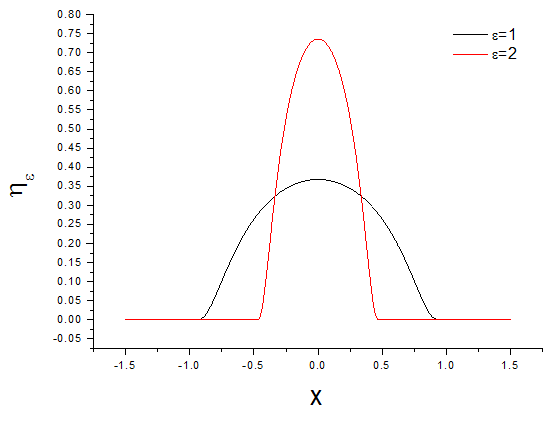
\includegraphics[width=0.5\textwidth]{kernel}
\end{figure}
\s

We have that $\eta_{\epsilon}(x) \in C^{\infty}(\reals^n)$ and $\text{supp}(\eta_{\epsilon}) \subset B_{\epsilon}(0)$.
\end{itemize} 
\s

We let $U_{\epsilon} = \{ x\in U | \text{dist}(x,\partial U) > \epsilon \}$.
\s

\defi If $f: U\rightarrow \reals^n$ is locally integrable. i.e. $f\in L^1_{\text{loc}}(U)$. We define its $\epsilon$-mollification $f^{\epsilon} : U_{\epsilon} \rightarrow \reals$ by $f^{\epsilon} = \eta_\epsilon * f$, i.e.
\begin{align*}
f^{\epsilon}(x) = \int_U \eta_{\epsilon}(x-y) f(y)dy
\end{align*}
\s

Think of this as the average of $f$ in a neighbourhood of $x$, weighted by $\eta_{\epsilon}$ shifted to have its peak at $x$.
\s

\thm (Properties of Mollifiers) \begin{itemize}
\item[(i)] $f^{\epsilon} \in C^{\infty}(U_{\epsilon})$ and $D^{\alpha}f^{\epsilon} = \int_U D^{\alpha}_x \eta_{\epsilon}(x-y)f(y) dy$.
\item[(ii)] $f^{\epsilon}\rightarrow f$ almost everywhere as $\epsilon \rightarrow 0$.
\item[(iii)] If $f\in C^0 (U)$, then $f^{\epsilon} \rightarrow f$ uniformly on compact subsets of $U$.
\item[(iv)] If $1\leq p <\infty$ and $f \in L^p_{\text{loc}}(U)$ then $f^{\epsilon} \rightarrow f$ in $L^p_{\text{loc}}(U)$, i.e.
\begin{align*}
\norms{f^{\epsilon} - f}{L^p(V)} \rightarrow 0 \quad \forall V \subset\subset U
\end{align*}
\end{itemize}
\begin{proof}
\pf See handout
\end{proof}

\s

\lem Assume $u \in W^{k,p}(U)$ for some $1\leq p < \infty$. Set $u^{\epsilon} = \eta_{\epsilon} * u$ in $U_{\epsilon}$. Then
\begin{itemize}
\item[(i)] $u^{\epsilon} \in C^{\infty}(U_{\epsilon}) \quad \forall \epsilon >0$
\item[(ii)] If $V \subset \subset U$, then $u^{\epsilon} \rightarrow u$ in $W^{k,p}(V)$
\end{itemize}
\begin{proof}
\pf For (i), see handout.

For (ii), we claim $D^{\alpha} u^{\epsilon} = \eta_{\epsilon} * D^{\alpha} u$ for $|\alpha| \leq k$ in $U_{\epsilon}$, i.e. the derivative of $u^{\epsilon}$ is the $\epsilon$-mollifier of the derivative of $u$, i.e. derivatives commute with convolutions. To see this,
\begin{align*}
D^{\alpha} u^{\epsilon}(x) &= D^{\alpha} \int_U \eta_{\epsilon}(x-y) u(u) dy \\
&= \int_U D_x^{\alpha} \eta_x(x-y) u(y) dy \\
&= (-1)^{|\alpha|} \int_U D_y^{\alpha} \eta_x(x-y) u(y) dy \\
&= \int_U \eta_{\epsilon}(x-y) D^{\alpha} u(y) dy \quad \quad \text{(by definition of weak derivatives)} \\
&= \eta_{\epsilon} * D^{\alpha} u(x)
\end{align*}
Now, fix $V\subset \subset U$. By previous theorem, $\eta_{\epsilon} * D^{\alpha} u \rightarrow D^{\alpha} u$ in $L^p_{\text{loc}}(U)$. So $D^{\alpha} u^{\epsilon} \rightarrow D^{\alpha} u$. in $L^p_{\text{loc}}(U)$ for all $|\alpha| \leq k$. Thus :
\begin{align*}
\norms{u^{\epsilon}- u}{W^{k,p}(V)}^p = \sum_{|\alpha|\leq k} \norms{D^{\alpha} u^{\epsilon} - D^{\alpha}u}{L^p(U)}^p \rightarrow 0
\end{align*}
so indeed $u^{\epsilon} \rightarrow u$ in $W^{k,p}(U)$.

\eop
\end{proof}
\s

This tells us we can approximate $u$ in the interior of $U$ by smooth functions. We can do better :
\s

\thm (Global approximation by smooth functions) Suppose $U\subset \reals^n$ is open and \emph{bounded}, and suppose $u\in W^{k,p}(U)$ for some $1\leq p<\infty$. Then there exists functions $u_n \in C^{\infty}(U) \cap W^{k,p}(U)$ such that
\begin{align*}
u_n \rightarrow u \quad \text{in } W^{k,p}(U)
\end{align*}

Note, we do not assert $u_n \in C^{\infty}(\bar{U})$.
\begin{proof}
\pf \begin{itemize}
\item[1.] We have $U = \bigcup_{i=1}^{\infty} U_i$, where $U_i = \{x\in U \, : \, \text{dist}(x,\pa U) > 1/i \}$ for $i=1,2,\cdots$. Write $V_i = U_{i+3} \backslash \bar{U}_{i+1}$ and choose $V_0$ that is compact in $U$, so that we have $U = \bigcup_{i=1}^{\infty} V_i$. Let $\{\xi_i\}_{i=0}^{\infty}$ be a \emph{partition of unity subordinate} to $\{V_i \}$ so that
\begin{align*}
\begin{cases}
\xi_i \in C_c^{\infty}(V_i) \\
0\leq \xi_i \leq 1 \\
\sum_{i=0}^{\infty} \xi_i = 1 \quad \text{on } U
\end{cases}
\end{align*}
Suppose $u\in W^{k,p}(U)$. Then $\xi_i u \in W^{k,p}(U)$ and $\text{supp}(\xi_i u) \subset V_i$.
\item[2.] Fix $\delta >0$. For each $i$, choose $\epsilon_i$ sufficiently small that $u^i = \eta_{\epsilon_i} * (\xi_i u)$ satisfies
\begin{align*}
&\norms{u^i - \xi_i u}{W^{k,p}(U)} \leq \frac{\delta}{2^{i+1}} \quad i=0,1,2,\cdots \\
& \text{supp}(U_i) \subset W_i = U_{i+1} \backslash \bar{U}_i \quad i=1,2,\cdots
\end{align*}
\item[3.] Write $v = \sum_{i=0}^{\infty} u^i$, then $v \in C^{\infty}(U)$ as for each $V \subset\subset U$, the sum is finite. Since $u = \sum_{i=0}^{\infty} \xi_i u$, for each $V\subset\subset U$< we have
\begin{align*}
\norms{v-u}{W^{k,p}(U)} &\leq \sum_{i=0}^{\infty} \norms{u^i- \xi_i u}{W^{k,p}(U)} \\
& \leq \delta \sum_{i=0}^{\infty} 2^{-i-1} = \delta
\end{align*}
Take supremum over $V\subset\subset U$, and conclude $v \in W^{k,p}(U)$, and $\norms{v-u}{W^{k,p}(U)} \leq \delta$.
\end{itemize}

\eop
\end{proof}
\s

\newday

(26th October, Friday)
\s

\textbf{Last Lecture :} $U\subset \reals^n$ open and bounded, $u\in W^{k,p} (U) $, $1\leq  p<\infty$, there is a sequence $u_l \in C^{\infty}(U) \cap W^{k,p}(U)$ such that $u_l \rightarrow u$ in $W^{k,p}(U)$.
\s

However, if the boundary of $U$ is behaves badly, this approximation still is not good enough. We will extend this to an approximation result with $u_k \in C^{\infty}(\bar{U})$, but for this we require an assumption on $\pa U$.
\s

\defi Suppose $U\subset \reals^n$ is open and bounded, we say $U$ is a \textbf{$C^{k,\alpha}$ domain}, if for every $p\in \pa U = \bar{U} \backslash U$, there exists some $r>0$ and a $C^{k,\alpha}$ function $\gamma : \reals^{n-1} \rightarrow \reals$ such that (after possibly relabelling axes)
\begin{align*}
U \cap B_r (p) = \{ x\in B_{r}(p) : x_n > \gamma(x_1, \cdots, x_{n-1}) \}
\end{align*}
\begin{figure}[h]
	\centering
	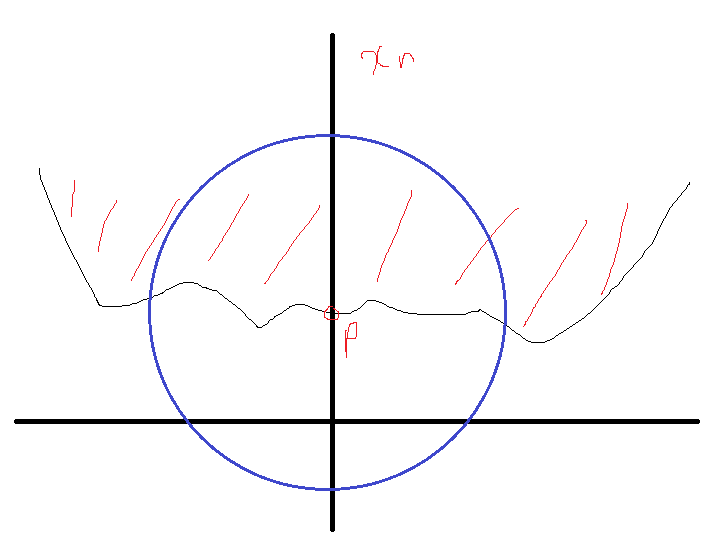
\includegraphics[scale=0.5]{2}
\end{figure}

\thm Suppose $U \subset \reals^n$ is a $C^{0,1}$ domain ($U$ has Lipshitz boundary). Let $u\in W^{k,p}(U)$ for some $1\leq p <\infty$. Then there exist functions $u_m \in C^{\infty}(\bar{U})$ such that $u_m \rightarrow u$ in $W^{k,p}(U)$.
\begin{proof}
\pf \begin{itemize}
\item[1.] Fix $x^0 \in \pa U$. Since $U$ is Lipshitz, $\exists r>0$, $\gamma \in C^{0,1}(\reals^{n-1})$ (after relabelling axes) s.t.
\begin{align*}
U \cap B_r(x^0) = \{ x\in B_r(x^0) : x_n > \gamma (x_1, \cdots, x_{n-1})\}
\end{align*}
Set $V = U \cap B_{r/2}(x^0)$.
\item[2. ] Define the shifted point $x^{\epsilon} = x+ \lambda \epsilon e_n$ ($x\in V, \epsilon >0$, $\lambda >0$, $e_n$ the unit vector in n-direction). For $\lambda$ large enough, $B_{\epsilon}(x^{\epsilon}) \subset U\cap B_r (x^0)$ for all $x\in V$ and $\epsilon$ small enough.
\begin{figure}[h]
	\centering
	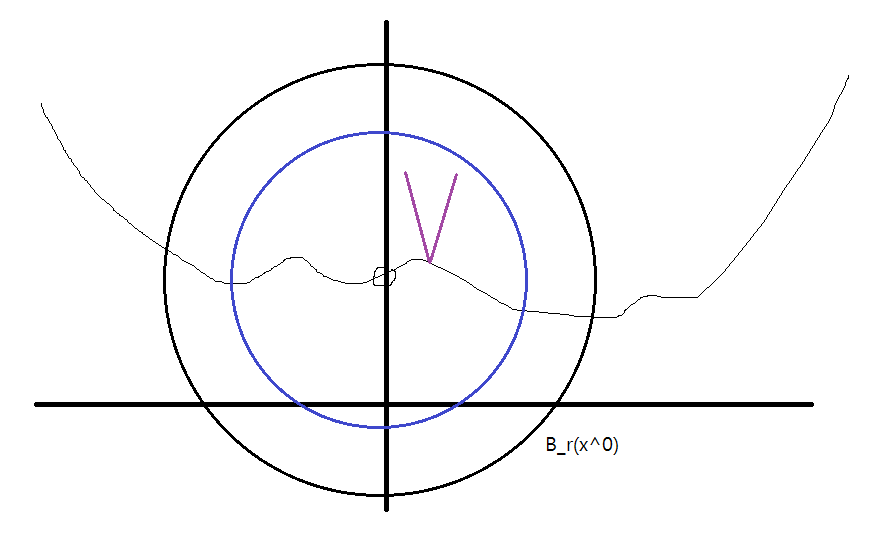
\includegraphics[scale=0.5]{3}
\end{figure}
This is equivalent to saying that above each point, we can find a cone which remains above the graph.  Also, we can choose $\lambda$ uniformly on $V$(e.g. $\lambda \geq \norms{\gamma}{C^{0,1}}$). Define
\begin{align*}
u_{\epsilon}(x) = u(x^{\epsilon}) \quad x\in V
\end{align*}
and set $v^{\epsilon,\tilde{\epsilon}} = \eta_{\tilde{\epsilon}} * u_{\epsilon}$ for $0 < \tilde{\epsilon} <\epsilon$. Clearly, we have $v^{\epsilon, \tilde{\epsilon}} \in C^{\infty}(\bar{V})$.
\item[3.] Fix $\delta >0$, we estimate
\begin{align*}
\norms{v^{\epsilon,\tilde{\epsilon}}-u}{W^{k,p}(V)} \leq \norms{v^{\epsilon,\tilde{\epsilon}}-u_{\epsilon}}{W^{k,p}(V)} + \norms{u_{\epsilon}-u}{W^{k,p}(V)}
\end{align*}
since translation is continuous in the $L^p$ norms, we can pick $\epsilon >0$ such that
\begin{align*}
\norms{u_{\epsilon}-u}{W^{k,p}(V)} < \delta /2
\end{align*}
Having fixed $\epsilon>0$, we can pick $\tilde{\epsilon}>0$ such that
\begin{align*}
\norms{v^{\epsilon,\tilde{\epsilon}}-u_{\epsilon}}{W^{k,p}(V)} < \delta /2
\end{align*}
by our previous theorem.
\item[4.] Now, since $\pa U$ is compact, we can find finitely main $x^0_i \in \pa U$ radii $r_i>0$, sets $V_i = U \cap B_{r_i /2}(x^0_i)$ and functions $v_i \in C^{\infty}(\bar{V}_i)$ for $i=1,\cdots,N$ satisfying
\begin{align*}
\norms{v_i - u}{W^{k,p}(V_i)} \leq \delta
\end{align*}
and $\pa U \subset \bigcup_{i=1}^N V_i$. Take an open $V_0 \subset \subset U$ such that $U \subset \bigcup_{i=0}^N V_i$ and by a previous result we can find $v_0 \in C^{\infty}_c(U)$ such that
\begin{align*}
\norms{v_0-u}{W^{k,p}(V_0)} \leq \delta
\end{align*}
\begin{figure}[h]
	\centering
	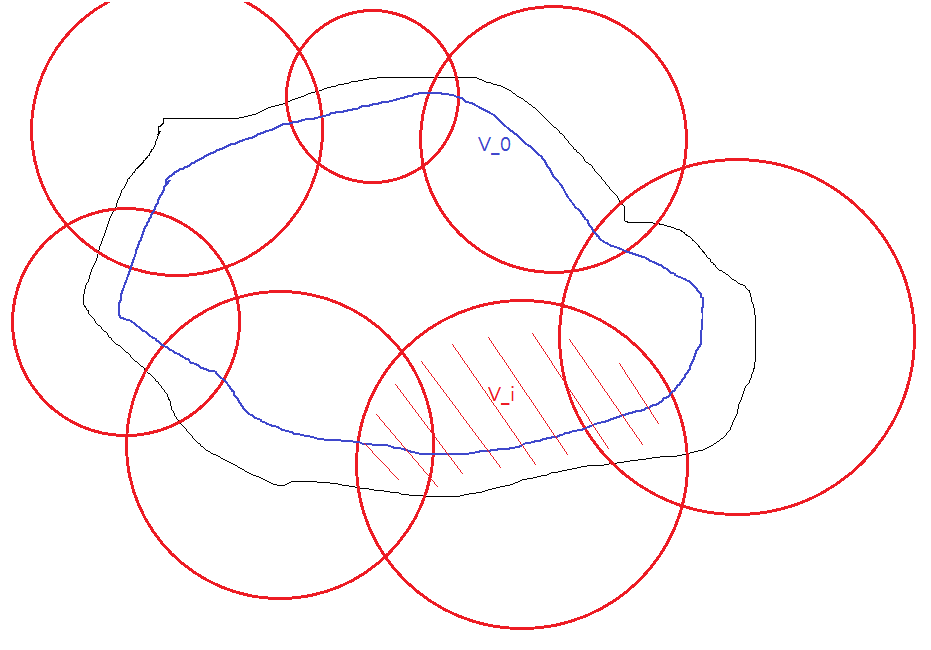
\includegraphics[scale=0.5]{4}
\end{figure}
\item[5.] Let $\{\xi_i\}_{i=0}^N$ be a smooth partition of unity subordinated to the open sets $\{V_0, \{B_{r_i/2}(x^0_i)\}_{i=1}^N \}$ such that $\xi_i \in C^{\infty}_c(B_{r_i/2}(x_i^0))$, $\xi_0 \in C_c^{\infty}(V_0)$, $0 \leq \xi_i \leq 1$ with $\sum_{i=0}^N \xi_i =1$ on $U$.

\quad Define $v = \sum_{i=0}^N \xi_i v_i$. Clearly $v \in C^{\infty}_c(\bar{U})$. Further, for $|\alpha|\leq k$,
\begin{align*}
\norms{D^{\alpha}v- D^{\alpha}u}{L^p(U)} &\leq \sum_{i=0}^N \norms{D^{\alpha}(\xi_i v_i) - D^{\alpha}(\xi_i u)}{L^p(V_i)} \\
&\leq C_k \sum_{i=0}^N \norms{v_i - u_i}{W^{k,p}(V_i)} \\
&\leq C_k (N+1)\delta
\end{align*}
As $\delta$ was arbitrary, we have the desired result.
\end{itemize}

\eop
\end{proof}
\s

\thm (Extension of Sobolev functions) Suppose $U\subset \reals^n$, open, bounded, is a $C^{1,0}$ domain. Choose a bounded $V$ such that $U \subset\subset V$. Then there exists a bounded linear operator $E : W^{1,p}(U) \rightarrow W^{1,p}(\reals^n)$ such that for each $u \in W^{1,p}(U)$ :
\begin{itemize}
\item[(i)] $Eu =u$ almost everywhere in $U$.
\item[(ii)] $Eu$ has support in $V$.
\item[(iii)] $\norms{Eu}{W^{1,p}(\reals^n)} \leq C \norms{u}{W^{1,p}(U)}$ where $C$ only depends on $U,V$ and $p$.
\end{itemize}
\s

We call $Eu$ an \textbf{extension of $u$ to $\reals^n$}. This is not unique.
\s

\lem Suppose $U = B_r(0) \cap \{x_n >0 \}$.  Suppose $u \in C^1( \overline{\{x_n>0 \}})$. We can find an $Eu \in C^1(\reals^n)$ such that
\begin{align*}
\norms{Eu}{W^{1,p}(B_r(0))} \leq C \norms{u}{W^{1,p}(U)}
\end{align*}
for some constant $C>0$.
\begin{proof}
\pf We define \begin{align*}
\bar{u}(x) = \begin{cases}
\begin{array}{lc}
u(x) & \text{if } x_n \geq 0 \\
-3u(x_1, \cdots, x_{n-1},-x_n) + 4u(x_1,\cdots, x_{n-1},\frac{-x_n}{2}) & \text{if } x_n<0
\end{array}
\end{cases}
\end{align*}
\begin{subproof}
\textbf{Claim :} $\bar{u} \in C^1(\reals^n)$.

\quad Clearly, $\bar{u} \in C^0(\reals^n)$ as
\begin{align*}
\lim_{x_n \rightarrow 0} -3u(x_1, \cdots,x_{n-1},-x_n) + 4u(x_1, \cdots, x_{n-1},-\frac{x_n}{2}) = u(x_1, \cdots, x_{n-1},0)
\end{align*}
Do similarly for $\pa_{x_j} \bar{u}$, $1\leq j\leq n-1$.

\quad For $x_n <0$,
\begin{align*}
\pa_{x_n} \bar{u}(x_1,\cdots, x_n) =& 3\pa_{x_n} u(x_1, \cdots, x_{n-1},-x_n) -2\pa_{x_n} u(x_1, \cdots, x_{n-1},-x_n/2)\\
& \rightarrow u_{x_n}(x_1, \cdots, x_{n-1},0) \quad \text{as } x_n \rightarrow 0^-
\end{align*}
So $U$, $Du$ are continuous across $\{x_n=0\}$. 
\end{subproof}
Setting $Eu = \bar{u}$, clearly $\bar{u}$ depends on $u$ linearly, and a computation shows $\norms{Eu}{W^{1,k}(U)} \leq C \norms{u}{W^{1,k}(U)}$

\eop
\end{proof}
\s

\newday

(29th October, 2018)
\s

Recall, we were on our way to proving the following theorem.
\s

\thm (Extension of Sobolev functions) Suppose $U\subset \reals^n$, open, bounded, is a $C^{1,0}$ domain. Choose a bounded $V$ such that $U \subset\subset V$. Then there exists a bounded linear operator $E : W^{1,p}(U) \rightarrow W^{1,p}(\reals^n)$ such that for each $u \in W^{1,p}(U)$ :
\begin{itemize}
\item[(i)] $Eu =u$ almost everywhere in $U$.
\item[(ii)] $Eu$ has support in $V$.
\item[(iii)] $\norms{Eu}{W^{1,p}(\reals^n)} \leq C \norms{u}{W^{1,p}(U)}$ where $C$ only depends on $U,V$ and $p$.
\end{itemize}
\s

Yet we need another lemma. Be aware that in the following lines of proof, the constant $C$ varies and might not indicate a single number.
\s

\lem Suppose $U\subset \reals^n$, bounded, open $C^1$-domain. Suppose $u\in C^1 (\bar{U})$. Then $\exists \bar{u} \in C^1_c(\reals^n)$ that depends linearly on $u$ and that
\begin{align*}
\norms{\bar{u}}{W^{1,p}(\reals^n)} \leq C \norms{u}{W^{1,p}(U)} \quad u= \bar{u} \text{ on } U
\end{align*}
\begin{proof} 
\pf We prove this lemma by reducing the setting to the setting of the previous lemma.
\begin{itemize}
\item[1.] Pick $x_0 \in \pa U$. After possibly relabelling axes, $\exists r>0$ such that
\begin{align*}
U \cap B_r(x_0) = \{x\in B_r(x_0) : x_n > \gamma(x_1, \cdots, x_{n-1}) \}
\end{align*}
for some $\gamma \in C^1(\reals^{n-1})$. (by definition of being a $C^1$-domain). Define $\Phi^i (x) = y^i$ where
\begin{align*}
& y^i  = x^i \quad \forall i=1, \cdots, n-1 \\
& y^n = x^n - \gamma(x^1, \cdots, x^{n-1})
\end{align*}
This has inverse $\Psi(y) = x$ where
\begin{align*}
& x^i = y^i \quad i=1,\cdots, n-1 \\
& x^n = y^n + \gamma(y^1, \cdots, y^{n-1})
\end{align*}
Clearly, $\Phi \circ \Psi = \Psi \circ \Phi = id_{B_r(x_0)}$,	
\begin{align*}
\Phi(U \cap B_r(x_0)) \subset \{y_0 >0 \}
\end{align*}
and $\Phi, \Psi$ are both $C^1$. If $y_0 = \Phi(X_0)$, $\exists s>0$ such that $B_s(y_0) \subset \Phi(B_r(x_0))$. Define $W = \Phi^{-1}(B_s(y_0))$.

\begin{figure}[h]
	\centering
	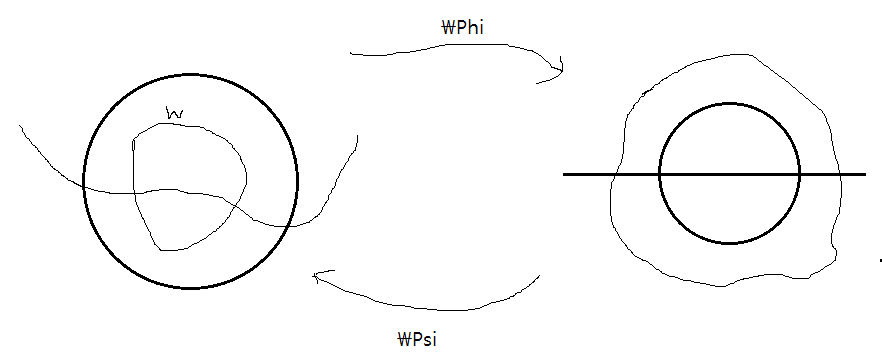
\includegraphics[width=0.5\textwidth]{5}
\end{figure}

\item[2.] For $y\in B_s(y_0) \cap \{y_n >0 \} = B_+$, we define
\begin{align*}
u'(y) = u(\Psi(y))
\end{align*}
By the previous lemma, $\exists \bar{u}' \in C^1 (B_s(y_0))$ such that $\bar{u}' = u'$ on $B_s(y_0) \cap \{y_0 >0\} = B_+$ and
\begin{align*}
\norms{\bar{u}'}{W^{1,p}(B_s(y_0))} \leq C \norms{u'}{W^{1,p}(B_+)}
\end{align*}
Converting back to $x$-coordinates, we define
\begin{align*}
\bar{u}(x) = \bar{u}' (\Phi(x)) \quad \forall x\in W. 
\end{align*}
Therefore $\bar{u}$ extends $u$ from $U\cap W$ to $W$ and (checking this is an exercise.)
\begin{align*}
\norms{\bar{u}}{W^{1,p}(W)} \leq C\norms{u}{W^{1,p}(U)}
\end{align*}
\item[3.] Since $\pa U$ is compact, we can take a finite number of points $x^i_0 \in \pa U$, open sets $W_i \ni x_0^i$ and extensions $\bar{u}_i$ of $u$ to $W_i$ such that $\bigcup_{i=1}^n W_i \supset \pa U$. Also, pick $W_0 \subset \subset U$ such that $\bigcup_{i=0}^N W_i \supset U$ and set $\bar{u}_0 =u$ on $W_0$.

\quad Pick a partition of unity subordinate to $\{w_i\}_{i=0}^N$, say $\{\xi_i \}_{i=0}^N$ such that (i) $\xi_i \in C_c^{\infty}(W_i)$, (ii) $0\leq \xi_i \leq 1$ and (iii) $\sum_{i=0}^N \xi_i(x) =1$ for all $x\in U$. Define
\begin{align*}
\bar{u} = \sum_{i=0}^N \xi_i \bar{u}_i
\end{align*}
Then if $x\in U$,
\begin{align*}
\bar{u}(x) = \sum_{i=0}^N \xi_i(x) u(x) = u(x)
\end{align*}
so $\bar{u} \in C_c^1(\reals^n)$ is an extension of $u$ and
\begin{align*}
\norms{\bar{u}}{W^{1,p}(\reals^n)} \leq C \norms{u}{W^{1,p}(U)}
\end{align*}
We can also check each step that $\bar{u}$ depends linearly on $u$. We write $\bar{u} = Eu$. 
\end{itemize}

\eop
\end{proof}
\s

We are finally ready to the prove the theorem based on the two previous lemmas.
\s

\begin{proof}
\textbf{proof of the extension theorem) }  Suppose $u \in W^{1,p}(U)$. By approximation theorem, $\exists u_m \in C^{\infty}(\bar{U})$ with $u_m \rightarrow u$ in $W^{1,p}(U)$ and a.e. In particular, the map $E$ of the previous lemmas is defined on each $u_m$. By linearity of $E$,
\begin{align*}
\norms{E(u_n - u_m)}{W^{1,p}(\reals^n)} = \norms{Eu_n - E u_m}{W^{1,p}(\reals^n)} \leq C\norms{u_n - u_m}{W^{1,p}(U)}
\end{align*}
Since $(u_n)_n$ is convergent in $W^{1,p}(U)$, it is Cauchy in $W^{1,p}(U)$, we deduce that $(Eu_m)_m$ is Cauchy in $W^{1,p}(\reals^n)$. Hence
\begin{align*}
E u_m \rightarrow \tilde{u}
\end{align*}
for some $F[u] \in W^{1,p}(\reals^n)$. In fact, $\tilde{u}$ is independent of approximating sequence so we set $Fu = \tilde{u}$ and linear in $u$. If needs be, we can always multiply our answer by $\phi \in C_c^{\infty}(U)$ with $\phi =1$ on $U$ to fix support on $Fu$. We can then check $F$ satisfies conditions (i),(ii) and (iii).

\eop
\end{proof}
\s

We can repeat our argument to show a result for extensions of functions in $W^{1,p}(U)$ where $U$ is a $C^k$ domain, using a suitable higher order reflections.
\s

\subsubsection*{Trace theorem}

Because Sobolev functions are defined only up to almost everywhere sense, we do not yet know what it means for a Sobolev function to be defined on a boundary of a domain(as a submanifold of codimension 1 has measure 0), which means that we can not state boundary value problems of PDEs properly. To amend this problem, we need the following trace theorem.
\s

\thm \emph{(Trace Theorem)} Assume $U\subset \reals^n$ is open, bounded $C^1$ domain. There exists a bounded linear operator
\begin{align*}
T : W^{1,p}(U) \rightarrow L^p(\pa U) \quad 1\leq p <\infty
\end{align*}
such that
\begin{itemize}
\item[(i)] $Tu = u \big|_{\pa U}$ if $u \in W^{1,p}(U) \cap C(\bar{U})$
\item[(ii)] $\norms{Tu}{L^p(\pa U)} \leq C\norms{u}{W^{1,p}(U)}$ for all $u\in W^{1,p}(U)$ where $C = C(U,p)$ only depends on $U$ and $p$.
\end{itemize}
\s

The operator $T$ allows us to talk about '\emph{the restriction of $u$ to $\pa U$}' even though $u$ is only defined almost everywhere, and $\pa U$ is a set of measure zero.
\begin{proof}
\pf \begin{itemize}
\item[(i)] First assume $u\in C^1(\bar{U})$, and as previously, suppose $x^0 \in \pa U$ and $\pa U$ is flat near $x^0$ lying in the plane $\{x_n =0\}$. Choose $B = B_r(x^0)$ for some $r>0$ such that
\begin{align*}
& B_+ = B \cap \{x_n \geq 0 \} \subset \bar{U} \\
& B_- = B \cap \{x_n \leq 0 \} \subset \reals^n \backslash U
\end{align*}
Set $\hat{B} = B_{r/2}(x^0)$, denote by $\Gamma$ the portion of $\pa U$ lying within $\hat{B}$. Pick $\xi \in C_c^{\infty}(B)$ such that $0\leq \xi \leq 1$ on $B$ and $\xi \equiv 1$ on $\hat{B}$. 
\begin{align*}
\int_{\Gamma} |u|^p dx'  &= \int_{\Gamma} \xi |u|^p dx' \quad \quad (dx' \text{ the area element of } \Gamma) \\
&\leq \int_{B\cap \{x_n =0\}} \xi |u|^p dx' \\
&\leq \int_{0}^r \frac{d}{dy_n} \Big[ - \int_{B\cap \{x_n = y_n \}} \xi |u|^p dx' \Big] dy_n \\
&= - \int_{B_+}  \pa_{x_n} \big(\xi |u|^p \big) dx \\
&= - \int_{B_+} \big( |u|^p \pa_{x_n}\xi  + p \pa_{x_n} u |u|^{p-1} \xi \big) dx
\end{align*}
Using Young's inequality($|ab| \leq |a|^p/p + |b|^q/q$), we have
\begin{align*}
\Big| (\pa_{x_n} u) |u|^{p-1} \Big| \leq \frac{|\pa_{x_n} u|^p}{p} + \frac{|u|^{q(p-1)}}{q} \quad \text{where } q = \frac{p}{1-p}
\end{align*}
and therefore
\begin{align*}
\int_{\Gamma} |u|^p dx' \leq C_{p,r} \int_{B^+} |u|^p + |Du|^p dx
\end{align*}
and therefore $\norms{u}{L^p(\Gamma)} \leq C_{p,r} \norms{u}{W^{1,p}(B_+)}$.
\end{itemize}
\end{proof}
\s

\newday

(31st October, Wednesday)
\s

\begin{proof}
\textbf{proof continued) } 

\textbf{Last lecture} : $U \subset \reals^n$ open, bounded, $\pa U$ is $C^1$. If $\pa U$ is flat near $x^0$ and $u\in C^{\infty} (\bar{Y})$. Then there exists open $\Gamma \subset \pa U$ such that
\begin{align*}
\int_{\Gamma} |u|^p dx' \leq C \int_U |u|^p + |Du|^p dx
\end{align*}
If $x^0 \in \pa U$, but $\pa U$ is not flat near $x^0$, we use a $C^1$ boundary straightening function as in the proof of the extension theorem to show $\exists \Gamma \subset \pa U$ open such that
\begin{align*}
\int_{\Gamma} |u|^p dS \leq C \int_{U} |u|^p + |Du|^p dx \quad 
\end{align*}
where $dS$ is area element of $\Gamma$ not in its original coordinate but in its parametrised coordinates. But by estimating the Jacobian of the chart, this can be replaced by the area element of $\Gamma$ without much difficulty.

\quad Use compactness of $\pa U$ with this result to show
\begin{align*}
\int_{\pa U} |u|^p dS \leq C\int_{Y} |u|^p + |Du|^p dx \quad \text{hence} \quad \norms{Tu}{L^p(\pa U)} \leq C\norms{u}{W^{1,p}(U)}
\end{align*}
(plus partition of unity as in the previous proofs)

\quad For general $u\in W^{1,p}(U)$, approximate by $u\in C^{\infty}(\bar{U})$. If $u\in W^{1,p}(U) \cap C^0(\bar{U})$ use that our approximating sequence converges uniformly to $u$ to show $Tu = u\big|_{\pa U}$.

(See the Example sheet 2 to fill in the gaps)
\end{proof}
\s

We have shown that associated to $u \in W^{1,p}(U)$ is $Tu \in L^p(\pa U)$, uniquely determined by $Tu=u\big|_{\pa U}$ for $u \in C^0(\bar{U})$. But it is not true that any $L^p$ function arises as a trace of some Sobolev function. That is, the \textbf{trace map} $T$ is not surjective. There exists $f \in L^p(\pa U)$ such that $Tu \neq f$ for all $u \in W^{1,p}(U)$.
\s

\textbf{Note :} Recall we defined $W_0^{1,p}$ to be the completion of $C_c^{\infty}$ in $W^{1,p}$-norm. So one can show without difficulty that if $u \in W_0^{1,p}(U)$ then $Tu=0$. The converse is true : if $u\in W^{1,p}(U)$ and $Tu =0$ then $u \in W_0^{1,p}(U)$. Finally, if $u\in W^{2,p}(U)$, $D_i u \in W^{1,p}(U)$ so one can define $u$ and $Du$ on $\pa U$ using $T$.
\s

\subsection*{Sobolev Inequalities, Embeddings}

(For this section, it would be useful to refer to Cl\'{e}ment's Analysis of Functions lecture notes)
\s

We can think of the $p$ in $L^p_{\text{loc}}$ as giving some measure of how 'spicky' the function can be. If $\gamma p <1$(or equivalently $\gamma <1/p$)
\begin{align*}
\norms{x^{-\gamma}}{L^p((0,1])}^p = \int_0^1 x^{-\gamma p} dx < \infty
\end{align*}
For larger $p$, the function must tend to infinity more slowly as $x\rightarrow 0$.
\s

The Sobolev embeddings tell us we can exchange 'differentiability' (i.e. $k$ in $W^{k,p}$), for 'integrability' (i.e. $p$ in $W^{k,p}$). The first result is:
\s

\thm \emph{(Sobolev-Gagliardo-Nirenberg, or SGN)} Assume $n>p$. We have $W^{1,p}(\reals^n) \subset L^{p^*} (\reals^n)$ with $p^* = \frac{np}{n-p}>p$, and $\exists C >0$ depending only on $n,p$ such that $\forall u \in W^{1,p}(\reals^n)$,
\begin{align*}
\norms{u}{L^{p^*}(\reals^n)} \leq C \norms{Du}{L^p(\reals^n)} \leq C\norms{u}{W^{1,p}(\reals^n)}
\end{align*}
\s

\lem Let $n\geq 2$ and $f_1, \cdots, f_n \in L^{n-1}(\reals^{n-1})$. For any $1\leq i\leq n$, denote $\tilde{x}_i = (x_1, \cdots, x_{i-1}, x_{i+1}, \cdots, x_n) \in \reals^{n-1}$ (remove $i^{\text{th}}$ component from $(x_1, \cdots, x_n) \in \reals^n$) and
\begin{align*}
f : \reals^n \rightarrow \reals \quad f(t) = f_1(\tilde{x}_1) f_2(\tilde{x}_2) \cdots f_n(\tilde{x}_n)
\end{align*}
Then $f\in L^1(\reals^n)$ with
\begin{align*}
\norms{f}{L^1(\reals^n)} \leq \prod_{i=1}^n \norms{f_i}{L^{n-1}(\reals^{n-1})}
\end{align*}
\begin{proof}
\pf We work by induction.

\quad For $n=2$, $f(x_1,x_2) = f_1(x_2)f_2(x_1)$ so
\begin{align*}
\norms{f}{L^1(\reals^n)} &= \int_{\reals^2} |f(x_1,x_2)| dx_1 dx_2 = \int_{\reals} |f_1(x_1)| dx_2 \int |f_2(x_2)| dx_1 \\
&= \norms{f_1}{L^1} \norms{f_2}{L^1}
\end{align*}

\quad Suppose result holds for some $n \geq 2$. Write $f(x_1, \cdots, x_{n+1}) = f_{n+1}(\tilde{x}_{n+1}) F(x)$, where $F(x)  = f_1(\tilde{x}_1) \cdots f_n(\tilde{x}_n)$ and note
\begin{align*}
\int_{y_1, \cdots, y_n} |f(y_1,\cdots, y_n, x_{n+1})| dy_1 \cdots dy_n \leq \norms{f_{n+1}}{L^n(\reals^n)} \norms{F(\cdot, x_{n+1})}{L^{n/(n-1)}(\reals^n)} \,\, \cdots (\dagger)
\end{align*}
by H\"{o}lder inequality. We apply the result for $n$ to $|f_1|^{n/(n-1)}(\cdot, x_{n+1}) \times \cdots \times |f_n|^{n/(n-1)}(\cdot, x_{n+1})$ to find
\begin{align*}
\norms{F(\cdot, x_{n+1})}{L^{n/(n-1)}(\reals^{n})} =& \norms{ |f_1|^{\frac{n}{n-1}}(\cdot, x_{n+1}) \times \cdots \times |f_n|^{\frac{n}{n-1}}(\cdot, x_{n+1})}{L^1(\reals^n)}^{\frac{n-1}{n}} \\
\leq & \Big( \prod_{i=1}^n \norms{ |f_i|^{n/(n-1)} (\cdot, x_{n+1}) }{L^{n-1}(\reals^{n-1})} \Big)^{n-1/n} \\
= & \prod_{i=1}^n \norms{f_i (\cdot, x_{n+1})}{L^n(\reals^{n-1})}
\end{align*}
Finally, we integrate ($\dagger$) over $x_{n+1}$ to get
\begin{align*}
\norms{f}{L^1(\reals^{n+1})} \leq & \norms{f_{n+1}}{L^n(\reals^n)} \int \prod_{i=1}^n \norms{f_i(\cdot, x_{n+1})}{L^n(\reals^{n-1})} dx_{n+1} \\
\leq & \norms{f_{n+1}}{L^n(\reals^n)} \prod_{i=1}^n \Big(  \int_{x_{n+1}} \norms{f_i}{L^n(\reals^{n-1})}^n (\cdot, x_{n+1}) dx_{n+1}  \Big)^{1/n} \quad \text{(by H\"{o}lder)} \\ 
= & \norms{f_{n+1}}{L^n(\reals^n)} \prod_{i=1}^n \norms{f_i}{L^n(\reals^n)}
\end{align*}
So result hold for $n+1$, so by induction we are done.

\eop
\end{proof}
\s

\begin{proof}
\textbf{proof of Sobolev-Gagliargo-Nirenberg in case $p=1$)} First assume $u\in C_c^{\infty}(\reals^n)$ since $u$ has compact support, we have
\begin{align*}
u(x) = \int_{-\infty}^{x_i} \pa_{x_i} u(x_1, \cdots, x_{i-1}, y, x_{i+1}, \cdots, x_n) dy
\end{align*}
so that
\begin{align*}
|u(x)| \leq \int_{-\infty}^{\infty} |Du(x_1, \cdots, x_{i-1},y,x_{i+1},\cdots, x_n)| dy
\end{align*}
Define $f_i(\tilde{x}_i)  = \int_{-\infty}^{\infty} |Du(x_1, \cdots, x_{i-1},y,x_{i+1},\cdots, x_n)| dy$. Thus
\begin{align*}
|u(x)|^{n/n-1} \leq \prod_{i=1}^n f_i(\tilde{x}_i)^{1/(n-1)}
\end{align*}
Integrating and using the previous lemma gives
\begin{align*}
\Big( \norms{u}{L^{n/(n-1)(\reals^n)}}  \Big)^{\frac{n-1}{n}} =& \norms{u^{\frac{n}{n-1}}}{L^1(\reals^n)}  \\
\leq& \prod_{i=1}^n \norms{f_i^{\frac{1}{n-1}}}{L^{n-1}(\reals^{n-1})} = \prod_{i=1}^n \norms{Du}{L^1}^{\frac{1}{n-1}} = \norms{Du}{L^1(\reals^n)}^{\frac{n}{n-1}}
\end{align*}
Since this estimate only depends on the size of $u$ and $Du$, by approximation by smooth functions, this also holds for $u\in W^{1,1}(\reals^n)$.

\eop
\end{proof}
\s

\newday

(2nd November, Friday)
\s

\textbf{Last lecture :}

\thm \emph{(Sobolev-Gagliardo-Nirenberg)} Assume $n>p$. We have $W^{1,p}(\reals^n) \subset L^{p^*} (\reals^n)$ with $p^* = \frac{np}{n-p}>p$, and $\exists C >0$ depending only on $n,p$ such that $\forall u \in W^{1,p}(\reals^n)$,
\begin{align*}
\norms{u}{L^{p^*}(\reals^n)} \leq C \norms{Du}{L^p(\reals^n)} \leq C\norms{u}{W^{1,p}(\reals^n)}
\end{align*}
\s

We proved $p=1$ case: $\norms{u}{L^{\frac{n}{n-1}}(\reals^n)} \leq \norms{Du}{L^1(\reals^n)}$, so the constant $C =1$. The trick in this proof was to combine the integrals in various directions in a good way, using a Lemma.

In the example sheet Exercise 2.12, we show that if the set $U$ has $C^1$ boundary, it satisfies an isoperimetric inequality, given an estimate of above form.
\s

\begin{proof}
\textbf{proof of the case $p>1$) } Now suppose $p>1$. We apply the $p=1$ result to $v= |u|^{\gamma}$ where $\gamma >1$ will be chosen later. We note the following fact from \textbf{Example sheet 2, Exercise 2.6}
\begin{subproof}
\textbf{Fact :} Suppose $U$ is bounded and $u\in W^{1,p}(U)$ for some $p\in [1,\infty)$. Also, let $F: \reals \rightarrow \reals$ is $C^1$ and $F'$ is bounded. Then $v(x)=F(u(x))$ is in $W^{1,p}(U)$ and the weak derivative is given by $\pa_{x_i} v = F'(u) \pa_{x_i u}$ for $i=1,\cdots,n$.
\end{subproof}
Hence, $v$ is weakly differentiable and 
\begin{align*}
Dv = \gamma \text{sign}(u) |u|^{\gamma -1} Du
\end{align*}
so
\begin{align*}
\norms{v}{L^{\frac{n}{n-1}}(\reals^n)} &= \Big( \int_{\reals^n} |u|^{\frac{\gamma n}{n-1}}  dx \Big)^{\frac{n-1}{n}} \leq \gamma \int_{\reals^n} |u|^{\gamma -1} |Du| dx \\
&\leq \gamma \Big( \int_{\reals^n} |u|^{(\gamma-1) \frac{p}{p-1}} dx \Big)^{\frac{p-1}{p}} \Big( \int_{\reals^n} |Du|^p dx \Big)^{1/p} \quad \text{(by H\"{o}lder)}
\end{align*}
We choose $\gamma$ such that
\begin{align*}
\frac{\gamma n}{n-1} = \frac{(\gamma -1)p}{p-1} \quad \Rightarrow \quad \gamma = \frac{p(n-1)}{n-p} >1
\end{align*}
Then $\frac{\gamma n}{n-1} = \frac{(n-1)p}{p-1} = \frac{np}{n-p} = p^*$ is as given in the statement of the theorem. Thus,
\begin{align*}
\Big( \int_{\reals^n} |u|^{p^*} dx \Big)^{1/p^*} = \frac{p(n-1)}{n-p} \Big( \int_{\reals^n} |Du|^p dx \Big)^{1/p}
\end{align*}

\eop
\end{proof}
\s

In fact, in the example sheet(Exercise 2.9), you will see that this family of inequality, bounding $\norms{u}{q}$ by $\norms{Du}{p}$, can only exist for only particular pair of exponents $(p,q)$ satisfying
\begin{align*}
\frac{1}{q} = \frac{1}{p} - \frac{1}{n}
\end{align*}
\s

\corrnum{1} Let $U \subset \reals^n$ be open, bounded $C^1$-domain, and $1\leq p<n$. Then $W^{1,p}(U) \subset L^{p^*}(U)$ (where $p^*$ is as before) and $\exists$ $C(p,n,U)$ such that
\begin{align*}
\norms{u}{L^{p^*}(U)} \leq C(p,n,U) \norms{Du}{W^{1,p} (U)} \quad \forall u \in W^{1,p}(U)
\end{align*} 
\begin{proof}
\pf By extension theorem, $\exists$ a bounded operator $E: W^{1,p}(U) \rightarrow W^{1,p}(\reals^n)$ such that $Eu = u$ on $U$ and $Eu$ has compact support. By Sobolev-Gagliardo-Nirenberg theorem, $Eu \in W^{1,p}(\reals^n)$ implies $Eu \in L^{p^*} (\reals^n)$ and therefore $u \in L^{p^*}(U)$ and
\begin{align*}
\norms{u}{L^{p^*}(U)} = \norms{Eu}{L^{p^*}(U)} \leq \norms{Eu}{L^{p^*}(\reals^n)} \leq C \norms{Eu}{W^{1,p}(\reals^n)} \leq \tilde{C}\norms{u}{W^{1,p}(U)}
\end{align*}

\eop
\end{proof}
\s

\corrnum{2} \emph{(Poincar\'{e} Inequality)} Suppose $U\subset \reals^n$ be open and bounded. Suppose $u \in W_0^{1,p}(U)$ for some $1\leq p<n$. Then we have the following estimate.
\begin{align*}
\norms{u}{L^q (U)} \leq C\norms{Du}{L^p(U)} \quad \forall q \in [1,p^*)
\end{align*}
where $C = C(p,q,n,U)$. In particular,
\begin{align*}
\norms{u}{L^{p}(U)} \leq C \norms{Du}{L^p(U)}
\end{align*}
\begin{proof}
\pf Since $u \in W^{1,p}_0(U)$, $\exists$ $u_m \in C_c^{\infty}(U)$ converging to $U$ in $W^{1,p}(U)$. Extend $u_m$ by zero on $U^c$ to get $\bar{u}_m \in C^{\infty}_c (\reals^n)$. Apply Sobolev-Gagliardo-Nirenberg inequality to find
\begin{align*}
\norms{u_m}{L^{p^*}(U)} \leq C \norms{Du_m}{L^p(U)}
\end{align*}
And further
\begin{align*}
\norms{u_m - u_{m'}}{L^{p^*}(U)} \leq C \norms{Du_m - Du_{m'}}{L^p(U)}
\end{align*}
Therefore, $(u_m)$ is Cauchy in $L^{p^*}(U)$, and hence $u_m$ converges in $L^{p^*}$. We can send $m\rightarrow \infty$ in $\norms{u_m}{L^{p^*}(U)} \leq C \norms{Du_m}{L^p(U)}$ further to find
\begin{align*}
\norms{u}{L^{p^*}(U)} \leq C \norms{Du}{L^p(U)}
\end{align*}

Since $\text{vol}(U) < \infty$, by H\"{o}lder, we can see that
\begin{align*}
\norms{u}{L^q(U)} \leq \norms{Du}{L^p(U)}  \quad \forall q \in [1,p^*]
\end{align*}
\eop
\end{proof}
\s

Now suppose $n<p< \infty$. Then naively, we might expect a function in $W^{1,p}(\reals^n)$ to be better than $L^{\infty}$. In fact, we have
\s

\thm \emph{(Morrey's Inequality)} Suppose $n<p<\infty$. Then $\exists C = C(p,n)$ such that
\begin{align*}
\norms{u}{C^{0,\gamma}(\reals^n)} \leq C\norms{u}{W^{1,p}(\reals^n)} \quad \forall u \in C_c^1(\reals^n)
\end{align*}
where $\gamma = 1-\frac{n}{p}$. (This can be interpreted as : as $p$ increases, we lose less and less information about differentiability in the Sobolev norm)
\begin{proof}
\pf We first establish the H\"{o}lder part of the estimate. Let $Q$ be an open cube, sides parallel to axes of side $r>0$ (centred at any point). Set
\begin{align*}
\bar{u} = \frac{1}{|Q|} \int_{Q} u(x) dx
\end{align*}
to be the average of $u$ on $Q$. Then
\begin{align*}
|\bar{u}-u(0)| = \Big| \frac{1}{|Q|} \int_{Q} u(x) -u(0) dx \Big| \leq \frac{1}{|Q|} \int_{Q} |u(x)-u(0)| dx
\end{align*}
Note
\begin{align*}
u(x) - u(0) = \int_0^1 \frac{d}{dt} u(tx)dx = \sum_{i=1}^n \int_0^1 x^i \frac{\pa u}{\pa x^i} (tx) dt
\end{align*}
so
\begin{align*}
|u(x) - u(0)| \leq r \int_0^1 \sum_{i=0}^n \Big| \frac{\pa u}{\pa x^i} (tx)\Big| dt \quad \text{(since }x\in Q \Rightarrow |x|<r)
\end{align*}
Thus
\begin{align*}
|\bar{u}-u(0)| &\leq \frac{r}{|Q|} \int_Q \int_0^1 \sum_{i=1}^n \Big| \frac{\pa u}{\pa x^i}(tx)\Big| dtdx  \\
&=\frac{r}{|Q|} \int_0^1 \Big( \int_Q \sum_{i=1}^n \Big| \frac{\pa u}{\pa x^i} (tx) \Big| dx \Big) dt \quad (\text{Fubini}) \\
&= \frac{r}{|Q|} \int_0^1 t^{-n} \Big( \int_{tQ} \sum_{i=1}^n \Big| \frac{\pa u}{\pa x^i} (y) dy \Big| dy \Big) dt \quad (y=tx) \\
&\leq \frac{r}{|Q|} \int_0^1 t^{-n} \Big( \sum_{i=1}^n \norms{\frac{\pa u}{\pa x^i}}{L^p(Q)} |tQ|^{1/p'} \Big) dt \quad (\text{H\"{o}lder}, \frac{1}{p}+ \frac{1}{p'} = 1)
\end{align*}
so using the fact $|Q| = r^n$ and $|tQ| = t^n r^n$,
\begin{align*}
|\bar{u}-u(0)| &\lesssim r^{1-n+ \frac{n}{p'}} \norms{Du}{L^p(\reals^n)} \int_0^1 t^{-n + \frac{n}{p'}} dt \\
&\lesssim \frac{r^{1-\frac{n}{p}}}{1-n/p} \norms{Du}{L^p(\reals^n)}
\end{align*}
Now suppose $x,y\in \reals^n$ with $|x-y| = r/2$. Pick a box containing $x,y$ with side $r$. By above,
\begin{align*}
|u(x) - u(y)| \leq |u(x)- \bar{u}| + |\bar{u} - u(y) | \lesssim \frac{r^{1-\frac{n}{p}}}{1-n/p} \norms{Du}{L^p(\reals^n)}
\end{align*}
and therefore
\begin{align*}
\frac{|u(x)-u(y)|}{|x-y|^{1-\frac{n}{p}}} \lesssim \frac{1}{1-n/p} \norms{Du}{L^p(\reals^n)}
\end{align*}
Finally, to see that $u$ is bounded for any $x\in \reals^n$, pick a box of side $1$ containing $x$ and estimate
\begin{align*}
|u(x)| \leq |\bar{u}-u(x)| + |\bar{u}| \lesssim \norms{Du}{L^p(\reals^n)} + \norms{u}{L^p(\reals^n)} \lesssim \norms{u}{W^{1,p}(\reals^n)}
\end{align*}

\eop
\end{proof}
\s

\newday

(5th November, Monday)
\s

\textbf{Last lecture :}
\begin{proof}
\thm \emph{(Morrey's Inequality)} Suppose $n<p<\infty$. Then $\exists C = C(p,n)$ such that
\begin{align*}
\norms{u}{C^{0,\gamma}(\reals^n)} \leq C\norms{u}{W^{1,p}(\reals^n)} \quad \forall u \in C_c^1(\reals^n)
\end{align*}
where $\gamma = 1-\frac{n}{p}$.
\end{proof}
\s

Morrey's inequality does not seem really useful at a first site. But from this, its follows a somewhat more useful and interesting result.
\s

\corr Let $n< p < \infty$. Suppose $u \in W^{1,p} (U)$. For $U\subset \reals^n$ open, bounded $C^{1}$-domain. (boundedness is in fact not necessary.) Then $\exists u^* \in C^{0,1-\frac{n}{p}}(U)$ such that $u = u^*$ almost everywhere, and
\begin{align*}
\norms{u^*}{C^{0,1-\frac{n}{p}}(U)} \leq C \norms{u}{W^{1,p}(U)}
\end{align*}
for some $C = C(n,p,U)$.
\begin{proof}
\pf By extension theorem, $\exists \bar{u} \in W^{1,p}(\reals^n)$ with $\bar{u} =u$ a.e. on $U$. We can find a sequence $u_m \in C_c^{\infty}(\reals^n)$ such that $u_m \rightarrow \bar{u}$ in $W^{1,p}(\reals^n)$ and $u_m(x) \rightarrow \bar{u}(x)$ for almost every $x$. By Morrey's inequality, has
\begin{align*}
\norms{u_m -u_{m'}}{C^{0,1-\frac{n}{p}}(\reals^n)} \leq C \norms{u_m - u_{m'}}{W^{1,p}(\reals^n)}
\end{align*}
and so $(u_m)_{m\geq 1}$ is Cauchy in $C^{0, 1-\frac{n}{p}}(\reals^n)$. Also, since $C^{0, 1-\frac{n}{p}}(\reals^n)$ is complete, $u_m \rightarrow \bar{u}^*$ in $C^{0,1-\frac{n}{p}}(\reals^n)$. Hence $\bar{u}^* = \bar{u}$ almost everywhere, so $u^* = \bar{u}^* \big|_{U}$. This satisfies our conditions.

\eop
\end{proof}
\s

\begin{tabular}{|p{0.9\textwidth}|}
\hline\\
The following diagram abstracts what we had been doing :

\begin{center}
\begin{large}
\begin{tikzcd}
{} & u \in W^{1,p}(\reals^n) \arrow[rd, "n<p"] \arrow[ld, "n>p"] & {} \\
u \in L^{p^*}(\reals^n)
& {} &  u\in C^{0,1-\frac{n}{p}}(\reals^n)
\end{tikzcd}
\end{large}
\end{center}
where the left arrow is implied by SGN inequality and the right arrow is implied by the corollary right above.
\\\\\hline
\end{tabular}
\s

By iterating these results, it is possible to establish similar embedding results for $W^{k,p}(\reals^n)$ into $W^{k',p'}(\reals^n)$ for $k'<k, p'>p$ or $C^{k',\gamma}(\reals^n)$ for $k'<k$.
\s

For example, we have $u \in W^{2,2}(\reals^3)$ $\Leftrightarrow$ $Du \in W^{1,2}(\reals^3)$ and $u \in W^{1,2}(\reals^3)$. This implies $Du \in L^6(\reals^3)$ and $u\in L^6(\reals^3)$, and therefore $u\in W^{1,6}(\reals^3)$ and finally $u \in C^{0,1/2}(\reals^3)$ by the corollary.
\s

\section*{Second Order Elliptic Equations}

Let $U\subset \reals^n$ and consider the operator
\begin{align*}
Lu = - \sum_{i,j=1}^n \big( a^{ij}(x) u_{x_j} \big)_{x_i} + \sum_{i=1}^n b^i (x) u_{x_i} + c(x)u \quad (\textbf{Divergence form})
\end{align*}
where $a^{ij},b^i,c$ are given functions on $U$. Typically we will assume they are at least $L^{\infty}$, but sometimes we will require more. 

\quad Assuming $a^{ij} \in C^{1}(U)$ we can write $L$ in \textbf{non-divergence form} as
\begin{align*}
Lu = -\sum_{i,j=1}^n a^{ij}u_{x_i x_j} + \sum_{i=1}^n \tilde{b}^i u_{x_i} + cu 
\end{align*}
where $\tilde{b}^i = b^i - a^{ji}_{x_i}$.

\quad We further assume $L$ is elliptic. This implies that $L$ or $-L$ satisfies
\begin{align*}
\sum_{i,j} a^{ij} \xi_i \xi_j \geq 0 \quad \forall \xi \in \reals^n
\end{align*}
and has equality \emph{iff} $\xi=0$. This implies that every surface is non-characteristic. 
\s

It turns out this is not a strong enough condition in general. We shall also require \textbf{uniform ellipticity} :
\s

\defi $L$ is \textbf{uniformly elliptic} if $\exists \theta \in \reals_{>0}$ such that
\begin{align*}
0 \leq \theta |\xi|^2 \leq \sum_{i,j} a^{ij}(x) \xi_i \xi_j \quad \forall x\in U, \,\, \xi\in \reals^n
\end{align*}
\s

Uniform ellipticity is a statement about invertibility of matrix $(a_{ij})_{ij}$. In fact, in finite dimensional case, ellipticity implies uniform ellipticity.
\s

We consider the boundary value problem
\begin{align}
\begin{cases} 
Lu = f \quad \text{in } U \\
u\big|_{\pa U} =0
\end{cases} \label{12}
\end{align} 
where $U$ is \emph{always} open bounded $C^1$-domain.
\s

\textbf{Example :} Let $L=-\Delta$, then the above problem models the electrostatic potential $u$, sourced by a charge distribution $f$, inside a cavity $U$ whose walls are grounded.
\s

It will turn out that form (\ref{12}) is not so well suited to finding solutions. We shall reformulate the problem into a more amenable form.

\quad Suppose $u\in C^2(\bar{U})$ is a solution of
\begin{align*}
Lu = - \sum_{i,j=1}^n \big( a^{ij}(x) u_{x_j} \big)_{x_i} + \sum_{i=1}^n b^i (x) u_{x_i} + c(x)u = f
\end{align*}
with $u=0$ on $\pa U$. Multiplying these equation by $v\in C^2(\bar{U})$ satisfying $v=0$ on $\pa U$, we find :
\begin{align*}
\int_U vLu dx = \int_U (-v) \sum_{i,j=1}^n \big( a^{ij}(x) u_{x_j} \big)_{x_i} + v\sum_{i=1}^n b^i (x) u_{x_i} + c(x)u v dx = \int fv dx
\end{align*}
Now, by the divergence theorem,
\begin{align*}
\int_U -\sum_{i,j} v\big(a^{ij}u_{x_j}\big)_{x_i} dx &= - \int_{\pa U} v \sum_{i,j} a^{ij} u_{x_j} dS_i + \int_U \sum_{i,j} a^{ij} u_{x_i} v_{x_j} \\
&= \int_U \sum_{i,j} a^{i,j} u_{x_j} v_{x_i}
\end{align*}
If we define $B[u,v] = \int_U \sum_{i,j} a^{ij}(x) u_{x_j} v_{x_i} + \sum_{i} b^i u_{x_i} v + cu\cdot v dx$, we deduce 
\begin{align*}
B[u,v] &= \int_U \sum_{i,j} a^{ij}(x) u_{x_j} v_{x_i} + \sum_{i} b^i u_{x_i} v + cu\cdot v dx \\
&= \int_U fv dx = \big(f,v \big)_{L^2(U)} 
\end{align*}
Conversely, suppose $u\in C^2(\bar{U})$ satisfies $u\big|_{\pa U} = 0$ and
\begin{align*}
B[u,v] = \big( f,v \big)_{L^2(U)} \quad \forall v \in C^2(\bar{U}), \,\, v\big|_{\pa U} =0
\end{align*}
We can undo the integration by parts to deduce
\begin{align*}
\int_U (Lu -f) v dx =0 \quad \forall v \in C^2(\bar{U}), \,\, v\big|_{\pa U} =0
\end{align*}
implies $Lu=f$.
\s

We conclude :

\quad $u \in C^2(\bar{U})$ with $u \big|_{\pa U} =0$ solves (\ref{12}) \emph{if and only if}
\begin{align*}
B[u,v] = \big( f,v \big)_{L^2(U)} \quad \text{with} \quad v\big|_{\pa U} = 0
\end{align*}
\s

Note that $B[u,v]$ in fact makes sense for $u,v\in H^1(U)$. To encode the boundary conditions, we can require $u,v$ vanish on $\pa U$ in the \emph{trace sense}(as in the trace theorem), or equivalently $u,v \in H_0^1(U)$. This motivates us to define \textbf{weak solution} of a PDE.
\s

\defi We say that $u\in H^1_0(U)$ is a \textbf{weak solution} of the problem
\begin{align*}
\begin{cases}
\begin{array}{ll}
Lu = f & \text{in } U \\
u =0 & \text{on } \pa U
\end{array}
\end{cases}
\end{align*}
For $y\in L^2(U)$ given, if
\begin{align*}
B[u,v] = \big( f,v \big)_{L^2(U)} \quad \forall v\in H_0^1 (U)
\end{align*}
\s

A synopsis for existential proof of a PDE : will first show that weak solutions always exist, and provided sufficient smoothness of $f$, the weak solution is in fact smooth.
\s

\newday

(7th November, Wednesday)
\s

(Example class 8th November, Thursday) - group A : 2:30 - 4:00, group B : 4:00 - 5:30 pm
\s

To prove existence of weak solutions, we use some structure of Hilbert spaces. Here, we assume some results from Part II Linear Analysis course, or any first course in functional analysis.
\s

\thm \emph{(Lax-Milgram)} Let $H$ be a (real) Hilbert space, with inner product $(\cdot, \cdot)$ and suppose
\begin{align*}
B : H\times H \rightarrow \reals
\end{align*}
is a bilinear mapping such that $\exists$ $\alpha, \beta >0$ such that
\begin{itemize}
\item[(i)] (\textbf{Boundedness}) $|B[u,v]| \leq \alpha \norms{u}{} \norms{v}{}$ for all $u,v \in H$. 
\item[(ii)] (\textbf{Coercivity}) $\beta \norms{u}{}^2 \leq B[u,v]$ for all $u \in H$ 
\end{itemize}
Finally, let $f: H\rightarrow \reals$ be a bounded linear functional on $H$. Then there exists a unique $u\in H$ such that
\begin{align*}
B[u,v] = \langle f, v\rangle \quad \forall v \in H
\end{align*}
(Here, $\langle f,v\rangle$ means $f(v)$ is a pairing of $H$ with its dual).
\begin{proof}
\pf \begin{itemize}
\item[1.] For each fixed $u\in H$, the map $v\mapsto B[u,v]$ is a bounded linear functional on $H$, so by the \emph{Riesz representation theorem}, $\exists$ unique $w\in H$ satisfying
\begin{align}
B[u,v] = (w, v) \quad \forall v \in H \label{13}
\end{align}
We write $Au =w$ when (\ref{13}) holds, so that
\begin{align*}
B[u,v] = (Au,v) \quad \forall u,v\in H
\end{align*}
\item[2.] We claim $A: H\rightarrow H$ is a bounded linear operator. If $\lambda_1, \lambda_2 \in \reals$, $u_1, u_2 \in H$ then for all $v\in H$, we compute
\begin{align*}
\big( A(\lambda_1 u_1 + \lambda_2 u_2), v \big) &= B[\lambda_1 u_1 + \lambda_2 u_2, v] = \lambda_1 B[u,v] + \lambda_2[u_2,v] \\
& = \lambda_1(Au,v) + \lambda_2 (Au_2, v) = (\lambda_1 Au_1 + \lambda_2 Au_2, v)
\end{align*}
Since $v$ was arbitrary, we have $A(\lambda_1 u_1 + \lambda_2 u_2) = \lambda_1 A u_1 + \lambda_2 Au_2$. Further,
\begin{align*}
\norms{A u}{}^2 = (Au, Au) = B[u,Au] \leq \alpha \norms{u}{} \norms{Au}{}
\end{align*}
so $A$ is bounded.
\item[3.] Next, we assert : $A$ is injective and $A(H)$ is closed.
\begin{subproof}
\pf By coercivity, 
\begin{align*}
\beta \norms{u}{}^2 \leq B[u,u] = (Au,u) \leq \norms{Au}{} \norms{u}{}
\end{align*}
This implies $A$ is injective.

\quad For the second point, assume $(Au_m)_{m=1}^{\infty}$ is convergent. Then by the earlier estimate,
\begin{align*}
\beta \norms{u_m -u_{m'}}{} \leq \norms{Au_m - Au_{m'}}{}
\end{align*}
so $(u_m)_{m=1}^{\infty}$ is Cauchy in $H$, so $u_m \rightarrow u$ for some $u$. But since $A$ is bounded, it is continuous,
\begin{align*}
Au = A \lim_{m\rightarrow \infty} u_{m} = \lim_{m\rightarrow \infty} Au_m \in A(H)
\end{align*}
so $A(H)$ is closed.
\end{subproof}
\item[4.]  Now we show $A(H) =H$.
\begin{subproof}
\pf Since $A(H)$ is closed, we have
\begin{align*}
H = A(H) \oplus A(H)^{\perp}
\end{align*}
Suppose $w \in A(H)^{\perp}$. Then
\begin{align*}
0= (Aw,w) = B[w,w] \geq \beta \norms{w}{}^2
\end{align*}
and therefore $\norms{w}{} =0$. This tells us that $A(H)^{\perp}$ is trivial, and $H=A(H)$.
\end{subproof}
Putting two results together, $A$ has inverse $A^{-1} : H\rightarrow H$. Moreover, applying $\beta \norms{u}{} \leq \norms{Au}{}$ to $u=A^{-1}w$, we find
\begin{align*}
\norms{A^{-1} w}{}\leq \frac{1}{\beta} \norms{w}{}
\end{align*}
so $A^{-1}$ is bounded.
\item[5.] Now consider $f$ a bounded linear functional. By Riesz representation theorem, $\exists$ unique $w\in H$ such that
\begin{align*}
\langle f, v\rangle = (w,v) \quad \forall v\in H
\end{align*}
Let $u = A^{-1} w$. Then
\begin{align*}
B[u,v] = (Au,v) = (w,v) = \langle f,v\rangle \quad \forall v \in H
\end{align*}
\item[6.] Finally $u$ is unique :
\begin{subproof}
If $u, \tilde{u}$ both satisfy $B[u,v] =B[\tilde{u},v]= \langle f,v\rangle$ for all $v\in H$, then
\begin{align*}
B[u-\tilde{u}, v] =0 \quad \forall v\in H
\end{align*}
by bilinearity of $B$. Set $v= u-\tilde{u}$ so
\begin{align*}
0 = B[u-\tilde{u}, u-\tilde{u}] \geq \beta \norms{u-\tilde{u}}{} 
\end{align*}
and therefore $u=\tilde{u}$.
\end{subproof}
\end{itemize}
\eop
\end{proof}
\s

\subsection*{Energy Estimates}

Suppose $a^{ij}, b^i, c \in L^{\infty}(U)$ for $U$ open, bounded and let
\begin{align*}
B[u,v] = \int_U \Big[ \sum_{i,j} a^{ij}u_{x_i}v_{x_j} + \sum_i b^i u_{x_i} v + cu\cdot v \Big] dx
\end{align*}
for $U,v\in H_0^1 (U)$. Assume $a^{ij}$ satisfies the \emph{uniform ellipticity condition}.
\s

To apply Lax-Milgram theorem in a general setting, we nee some estimates related to boundedness and coercivity of $B$. 
\s

\thm There exist $\alpha, \beta >0$ and $\gamma \geq 0$ such that
\begin{itemize}
\item[(i)] $\big| B[u,v]\big| \leq \alpha \norms{u}{H^1(U)} \norms{v}{H^1(U)}$ for all $u,v\in H^1(U)$ \quad \emph{and}
\item[(ii)] $\beta \norms{u}{H^1(U)}^2 \leq B[u,u] + \gamma \norms{u}{L^2(U)}^2$ (\textbf{G{\aa}rding Inequality})
\end{itemize}
\begin{proof}
\pf \begin{itemize}
\item[(i)] We estimate
\begin{align*}
\big| B[u,v]\big| \leq \sum_{i,j} \norms{a^{ij}}{L^{\infty}(U)} \int_U |Du||Dv| dx + \sum_{i} \norms{b^i}{L^{\infty}(U)} \int_U |Du||v| dx + \norms{c}{L^{\infty}(U)} \int_U |u||v| dx
\end{align*}
so
\begin{align*}
\big| B[u,v]\big| &\leq c_1 \norms{Du}{L^2(U)} \norms{Dv}{L^2(U)} + c_2 \norms{Du}{L^2(U)} \norms{v}{L^2(U)} + c_3 \norms{u}{L^2(U)} \norms{v}{L^2(U)} \\
&\leq \alpha \norms{u}{H^1(U)} \norms{v}{H^1(U)}
\end{align*}
for some constants $c_1,c_2,c_3$ and $\alpha>0$.
\item[(ii)] Now use the uniform ellipticity to deduce, for some $\theta >0$,
\begin{align*}
\theta \int_U |Du|^2 dx &\leq \int_U \sum_{i,j} a^{ij}(x) u_{x_i} u_{x_j} dx \\
&= B[u,u] - \int_U \sum_{i=1}^n b^i u_{x_i} u + cu^2 dx \\
&\leq B[u,u] + \sum_{i=1}^n \norms{b^i}{L^{\infty}(U)} \int_U |Du||u| dx + \norms{c}{L^{\infty}} \int_U u^2 dx
\end{align*}
Now, by Young's inequality(or just AG inequality),
\begin{align*}
\int_U |Du||u| dx \leq \epsilon \int_U |Du|^2 dx + \frac{1}{4\epsilon} \int_U |u|^2 dx \quad \forall \epsilon>0
\end{align*}
Choosing $\epsilon$ small, we can arrange
\begin{align*}
\sum_i \norms{b^i}{L^{\infty}(U)} \int_U |Du||u| dx \leq \frac{\theta}{2} \int_U |Du|^2 dx + C \int_U u^2 dx
\end{align*}
Putting two inequalities together, we deduce
\begin{align*}
\frac{\theta}{2} \int_U |Du|^2 dx \leq B[u,u] + C \int_U u^2 dx
\end{align*}
whence
\begin{align*}
\beta \norms{u}{H^1(U)}^2 \leq B[u,u] + \gamma \norms{u}{L^2(U)}^2
\end{align*}
for some $\beta, \gamma\geq 0$.
\end{itemize}

\eop
\end{proof}
\s

Boundedness of $B$ follows from the first statement of the theorem, but we need some stronger conditions on $B$ to get coercivity from the second statement.
\s

\newday

(9th November, Friday)
\s

\textbf{Remark :} If $B[\cdot,\cdot]$ is a bilinear form corresponding to an operator with $b^i=0$, $c\geq 0$ then \emph{uniform ellipticity} immediately gives
\begin{align*}
\theta \int_U |Du|^2 dx \leq B[u,u]
\end{align*}
recall Poincar\'{e}'s inequality,
\begin{align*}
\norms{u}{L^2(U)} \leq C \norms{Du}{L^2(U)} \quad \forall u\in H_0^1 (U)
\end{align*}
We can deduce G{\aa}rding's inequality holds with $\gamma =0$ for $u\in H_0^1 (U)$ by modifying the above proof with choosing $\epsilon$ appropriately.
\s

\thm \emph{(First Existence Theorem for Weak Solutions)} Let $U\subset \reals^n$ be open, bounded and $L$ be as before. Then there exists $\gamma \geq 0$ such that for any $\mu \geq \gamma$ and any $f\in L^2(U)$ there exists a unique weak solution to the boundary value problem(BVP) :
\begin{align*}
\begin{cases}
\begin{array}{ll}
Lu + \mu u =f & \text{in } U  \quad \cdots\cdots (\dagger) \\
u = 0 & \text{on } \pa U
\end{array}
\end{cases}
\end{align*}
Moreover, $\norms{u}{H^1(U)} \leq C \norms{f}{L^2(U)}$ for some $C = C(L,U,\mu)$
\s

This tells us that the weak solution has an improved regularity compared to the source term $f$, and uniqueness of weak solution also follows from the last inequality.
\begin{proof}
\pf \begin{itemize}
\item[1.] Take $\gamma$ from G{\aa}rding's inequality for the blinear form $B$ corresponding to $L$. Let $\mu \geq \gamma$ and set
\begin{align*}
B_{\mu}[u,v] = B[u,v] + \mu (u,v)_{L^2(U)}
\end{align*}
This is the bilinear form associated to $L_{\mu}  = L+\mu$. By G{\aa}rding,
\begin{align*}
\beta \norms{u}{H^1(U)}^2 \leq B[u,u] + \gamma \norms{u}{L^2(U)}^2 \leq B_{\mu} [u,u]
\end{align*}
Also
\begin{align*}
|B_{\mu}[u,v]| \leq \tilde{\alpha}\norms{u}{H^1(U)} \norms{v}{H^1(U)}
\end{align*}
Thus $B_{\mu}$ satisfies hypotheses of Lax-Milgram with $H=H^1(U)$.
\item[2.] Fix $f\in L^2(U)$, for $v\in H^1(U)$. Define $\langle f,v\rangle = (f,v)_{L^2(U)}$. This is a bounded linear functional on $H^1_0(U)$. We apply Lax-Milgram to find a unique $u\in H_0^1(U)$ satisfying
\begin{align*}
B_{\mu}[u,v] = \langle f,v\rangle \quad \forall v\in H_0^1(U)
\end{align*}
This is precisely the condition that $u$ is a weak solution of ($\dagger$).
\item[3.] From G{\aa}rding, we have
\begin{align*}
\beta \norms{u}{H^1(U)}^2 \leq B_{\mu} (u,u) = (f,u)_{L^2(U)} \leq \norms{f}{L^2(U)} \norms{u}{L^2(U)}
\end{align*}
and therefore $\norms{u}{H^1(U)} \leq \frac{1}{\beta} \norms{f}{L^2(U)}$.
\end{itemize}

\eop
\end{proof}
\s

There is a couple of issues with this result :
\begin{itemize}
\item We would like to get rid of $\mu$.
\item We would like to know when our weak solution is actually a strong solution
\end{itemize}
\s

For a moment, consider the matrix problem of finding $u\in \reals^n$ such that
\begin{align*}
Au = f
\end{align*}
for $f\in \reals^n$, $A\in \text{Mat}(n\times n)$. If $\exists \gamma$ such that $A- \mu I$  is invertible for all $\mu \geq \gamma$, we can always solve $Au - \mu u =f$ for such $\mu$. However, in fact there are only finite number of values of $\mu$ such that $A - \mu I$ is not invertible - we want to do something similar in the case of solving PDEs. To do this, we need to have some knowledge on spectral theorem of linear operators.
\s

An important concept in the study of PDEs is the idea of compactness. We can often find a bounded sequence (say of approximations to the solution of some PDE) and we would like to extract a subsequence which converges, e.g. \emph{Bolzanno-Weierstrass theorem}
\s

\defi Suppose $(U_n)_{n=1}^{\infty}$ is a sequence in a Hilbert space $\big( H,(\cdot,\cdot) \big)$. We say that $u_n$ converges \textbf{weakly} to $u\in H$, written $u_n \rightarrow u$ if
\begin{align*}
(u_n, w) \rightarrow (u,w) \quad \forall w\in H
\end{align*}
A weak limit, if it exists, is unique.
\s

\thm Let $H$ be a separable Hilbert space and suppose $(u_n)_{n=1}^{\infty}$ is a bounded sequence, $u_n \in H$, $\norms{u_n}{} \leq K$ for all $n$. Then $(u_n)_{n=1}^{\infty}$ admits a weakly convergent subsequence.
\begin{proof}
\pf Let $(e_i)_{i=1}^{\infty}$ be an orthonormal basis for $H$. Consider $(e_1, u_n)$. We have
\begin{align*}
|(e_1, u_n)| \leq \norms{e_1}{} \norms{u_n}{} \leq K
\end{align*}
so by Bolzonno-Weierstrass, $\exists (n_k)_{k} \subset \mathbb{N}$ such that $(e_1, u_n) \rightarrow c_1$ with $|c_1| \leq K$. We set $u_{1,j} = u_{n_j}$. Repeating the same argument with $(e_2, u_{1,j})$ we deduce $\exists j_k$ such that $(e_2, u_{1,j_k}) \rightarrow c_2$ with $|c_2| \leq K$. Set $u_{2,k} = u_{1,j_k}$. Continue inductively to define $u_{l,m}$ where $(u_{l+1,m})_{m=1}^{\infty}$ is a subsequence of $(u_{l,m})_{m=1}^{\infty}$ and such that $(e_j, u_{l,m}) \rightarrow c_j$ as $m\rightarrow \infty$ for all $j\leq l$ where $|c_j| \leq K$. Now consider a diagonal sequence $(u_{l,l})_{l=1}^{\infty}$. This is a subsequence of $(u_m)_{m=1}^{\infty}$ and $(e_j, u_{l,l}) \rightarrow c_j$ for all $j$ as $l\rightarrow \infty$ with $|c_1| \leq K$.
\end{proof}
\s

\newday

(12th November, Monday)
\s

\begin{proof}
\textbf{proof continues)} Last lecture we constructed a subsequence $(u_{m_j})_{j=1}^{\infty}$ such that
\begin{align*}
(e_i, u_{m_j}) \rightarrow c_i \quad\quad \text{with } |c_i| \leq K \quad \forall i=1,2,\cdots
\end{align*}
where $\{e_j \}$ is an o.n. basis. After relabelling, assume $(e_i ,u_m) \rightarrow c_i$ for $i=1,2\cdots$.
\s

Consider 
\begin{align*}
\sum_{j=1}^p |c_j|^2 &= \lim_{m\rightarrow \infty} \sum_{j=1}^p |(e_j, u_m)|^2 \leq \sup_{m} \sum_{j=1}^p |(e_j, u_m)|^2 \\
&\leq  \sup_{m} \norms{u_m}{}^2 \leq K^2
\end{align*}
so $\sum_{j=1}^{\infty} |c_j|^2$ converges, hence $u= \sum_{j=1}^{\infty} c_j e_j$ defines an element of $H$ and $\norms{u}{} \leq K$. We have
\begin{align*}
(e_j, u_m) \rightarrow (e_j, u) \quad \forall j
\end{align*}
It remains to show that $(w, u_m) \rightarrow (w,u)$ for any $w\in H$.
\begin{subproof}
: to see this, for $w\in H$ write
\begin{align*}
w= \sum_{i=1}^p (w,e_j) e_j + w_p \quad p\in \mathbb{N}
\end{align*}
Note $w_p \rightarrow 0$ as $p\rightarrow \infty$. We consider
\begin{align*}
(w,u_m) - (w,u) = (w-w_p, u_m -u) + (w_p, u_m-u)
\end{align*}
By Cauchy-Schwarz, has $|(w_p, u_m -u)| \leq \norms{w_p}{} \norms{u_m -u}{} \leq 2K \norms{w_p}{} < \epsilon/2$ for sufficiently large $p$. Now $w-w_p$ is a finite combination of $e_j$'s, so for $m$ large enough, $|(w-w_p, u_m -u)| < \epsilon/2$.
\end{subproof}

\eop
\end{proof}

This fact is important and useful, but we shall require a slightly stronger version which tells us that a bounded sequence in $H^1$ has a subsequence which converges strongly in $L^2(U)$ for $U$ bounded.
\s

First we revisit Poincar\'{e} :
\s

\lem \emph{(Poincar\'{e} revisited)} Suppose $u\in H^1(\reals^n)$. Let
\begin{align*}
Q = [\xi_1, \xi_1 +L] \times [\xi_2, \xi_2 +L] \times \cdots \times [\xi_n, \xi_n +L]
\end{align*}
be a cube of side length $L$. Then we have:
\begin{align*}
\norms{u}{L^2(Q)}^2 \leq \frac{1}{|Q|} \Big( \int_Q udx \Big)^2 + \frac{n}{2} |L|^2 \norms{Du}{L^2(Q)}^2
\end{align*}
\s

Note, this is equivalent to saying $\norms{u - \overline{u}}{L^2(Q)}^2 \leq \frac{n}{2} |L|^2 \norms{Du}{L^2(Q)}^2$ where $\overline{u} = \frac{1}{|Q|} \int_Q u(x) dx$ - which makes explicit connecting with Poincar\'{e} inequality.
\s

\begin{proof}
\textbf{(This proof is written as done in the lecture but is faulty - correct proof is followed right after this)}
\s

\textbf{proof of Lemma)} By approximation, assume $u\in C^{\infty}(\bar{Q})$. By convexity of $Q$ plus Fundamental Theorem of Calculus,
\begin{align*}
u(x) -u(y) = \int_0^1 \frac{d}{dt} u(tx + (1-t)y) dt = \int_0^1 (x-y) \cdot Du(tx + (1-t)y) dt
\end{align*}
Squaring and using Cauchy-Schwartz, obtains
\begin{align*}
u(x)^2 + u(y)^2 - 2u(x) u(y) \leq \int_0^1 |x-y|^2 |Du(tx + (1-t)y)|^2 dt
\end{align*}
Integrating $dx dy$ over $Q$ and using the fact that $|x-y| \leq nL^2$ for $x,y\in Q$, gets
\begin{align*}
2|Q| \norms{u}{L^2(Q)}^2 -2 \Big( \int_Q u(x) dx\Big)^2 &\leq nL^2 \int_Q \int_Q \int_0^1 |Du(tx + (1-t)y)|^2 dtdxdy \\
&= nL^2 \int_Q  \int_0^1 dt \int_{Qt} |Du(\zeta)|^2 d\zeta dtdy \quad \quad  (x = \zeta - (1-t)y/t) \\
&= nL^2 |Q| \times 1 \times \norms{Du}{L^2(Q)}^2
\end{align*}
Result follows on rearranging.

\eop
\end{proof}
\s

\begin{proof}
\textbf{(This proof is the corrected proof. Handout was distributed on 16th November, Friday)}
\s

\textbf{proof of Lemma)} By approximation, we can assume $u\in C^{\infty}(\overline{Q})$. For $x,y\in Q$ we use the fundamental theorem of calculus to write
\begin{align*}
u(x)-u(y) = \int_{y_1}^{x_1} \frac{d}{dt} u(t,x_2, \cdots, x_n) dt &+ \int_{y_2}^{x_2} \frac{d}{dt} u(y,t,x_3, \cdots, x_n) dt \\
& + \cdots + \int_{y_n}^{x_n} \frac{d}{dt} u(y_1, \cdots, y_{n-1},t)dt
\end{align*}
Squaring this identity, we have
\begin{align*}
u(x)^2 + u(y)^2 - 2u(x)u(y) \leq & n \Big( \int_{y_1}^{x_1} \frac{d}{dt} u(t,x_2, \cdots, x_n)dt \Big)^2 \\
& + \cdots + n\Big( \int_{y_n}^{x_n} \frac{d}{dt} u(y_1, \cdots, y_{n-1},t)dt \Big)^2 \quad \cdots \cdots \cdots \textbf{(A)}
\end{align*}
where on the RHS we have use $(a_1 + \cdots + a_n)^2 \leq n(a_1 + \cdots + a_n^2)$ which follows from Cauchy-Schwarz inequality. Integrating the above inequality over $x$ and $y$ in $Q$ gives
\begin{align*}
\int_Q dx \int_Q dy (u(x)^2 + u(y)^2 -2u(x)u(y)) = 2|Q|\norms{u}{L^(Q)}^2 -2 \Big( \int_Q u(x) dx \Big)^2
\end{align*}
Now consider
\begin{align*}
I_1 = \Big( \int_{y_1}^{x_1} \frac{d}{dt} u(t,x_2, \cdots, x_n) dt\Big)^2 &\leq \Big( \int_{y_1}^{x_1} dt\Big) \Big( \int_{y_1}^{x_1} (\frac{d}{dt}u(t,x_2, \cdots, x_n))^2 \Big) \\
&\leq L \int_{\xi_1}^{\xi_1 +L} (\frac{d}{dt} u(t,x_2\cdots,x_n))^2 dt
\end{align*}
Again integrating over $x$ and $y$ in $Q$, we have
\begin{align*}
\int_Q dx \int_Q dy I_1 \leq L^2 |Q| \norms{D_1 u}{L^2(Q)}^2
\end{align*}
where the extra factor of $L(Q)$ arises due to the integrand in independent of $y$ and $x_1$. Estimating the other terms on the RHS of (A) similarly yields
\begin{align*}
2 |Q| \norms{u}{L^2(Q)}^2 - 2 \Big( \int_Q u(x) dx\Big)^2 \leq nL^2 |Q| \times (\norms{D_1 u}{L^2(Q)}^2 + \cdots + \norms{D_n u}{L^2(Q)}^2)
\end{align*}
and the result follows on rearrangement.

\eop
\end{proof}


\thm \emph{(Rellich-Kondrachov)} Suppose $u \subset \reals^n$ is open, bounded $C^1$-domain. Let $(u_m)_{m=1}^{\infty}$ be a sequence in $H^1(U)$ with
\begin{align*}
\norms{u_m}{H^1(U)} \leq K
\end{align*}
Then there exists $u\in H^1(U)$ and a subsequence $(u_{m_j})_{j=1}^{\infty}$ such that $u_{m_j}$ tends to $u$ weakly in $H^1(U)$ and strongly in $L^2(U)$, i.e.
\begin{align*}
u_{m_j} \rightarrow u \quad \text{in } L^2(U), \quad u_{m_j} \xrightarrow{weak} u \quad \text{in } H^1(U)
\end{align*}

\textbf{Remark :} Could replace $H^1(U)$ with $H_0^1(U)$ everywhere and the result will hold. Then we could drop $C^1$ regularity of $\pa U$. 
\begin{proof}
\pf By extension theorem, we can assume $u_m \in H_0^1$ for some cube $Q$ with $U \subset \subset Q$. By the weak compactness result from earlier, $\exists u\in H_0^1(Q)$ and a subsequence $(u_{m_j})_{j=1}^{\infty}$ with $u_{m_j} \xrightarrow{w} u$ in $H_0^1(Q)$. Let $w_j = u_{m_j}$. We need to show $(w_j)_{j=1}^{\infty}$ converges in $L^2(Q)$.

\quad Fix $\epsilon >0$, pick $\delta >0$ that divides the side length of $Q$. We can cover $Q$ by $k(\delta)$ cubes, intersecting only on their faces with side lengths $(\leq)\delta$. Call these cubes $\{Q_a \}_{a=1}^{k(\delta)}$. Applying Poincar\'{e}'s inequality separately on each cube, we have
\begin{align*}
\norms{w_i - w_j}{L^2(Q)}^2 &= \sum_{a=1}^{k(\delta)} \norms{w_i -w_j}{L^2(Q_n)}^2 \\
& \leq  \sum_{a=1}^{k(\delta)} \Big[ \frac{1}{|Q_n|} \Big( \int w_i - w_j dx\Big)^2 + \frac{n^2 \delta^2}{2} \norms{Dw_i -Dw_j}{L^2(Q_n)}^2\Big] \\
& \leq \sum_{a=1}^{k(\delta)} \frac{1}{|Q_n|} \Big( \int w_i - w_j dx\Big)^2 + \frac{n^2 \delta^2}{2} \norms{Dw_i -Dw_j}{L^2(Q_n)}^2
\end{align*}
Note that $\frac{n^2 \delta^2}{2} \norms{Dw_i - Dw_j}{L^2(U)}^2 \leq C \frac{n^2\delta^2}{2} K^2$ where $C = C(U,Q)$ is the constant from extension, so for $\delta$ sufficiently small, 
\begin{align*}
\frac{n^2 \delta^2}{2}\norms{Dw_i - Dw_j}{L^2(U)}^2 < \epsilon/2
\end{align*}
- fix such $\delta$. Also, $u \mapsto \int_{Q_a} u(x)dx$ is a bounded linear functional on $H^1(Q)$ so since $w_j \xrightarrow{w} u$ in $H^1(Q)$, $(\int_{Q_n} w_i dx)_{i=1}^{\infty}$ is a Cauchy sequence. Since $k(\delta)$ is a fixed finite number, we conclude $\exists N$ such that if $i,j\geq N$ then
\begin{align*}
\sum_{a=1}^{k(\delta)} \frac{1}{|Q_n|} \Big( \int w_i - w_j dx\Big)^2 < \epsilon/2
\end{align*}
Putting these together, $\norms{w_i -w}{L^2(Q)}^2 < \epsilon$ for $i,j\geq N$. Thus $w_i$ is Cauchy, hence convergent in $L^2(Q)$. By uniqueness of weak limits, $w_i \rightarrow u$ in $L^2(Q)$.

\eop
\end{proof}
\s

\newday

(14th November, Wednesday)
\s

We will improve our existence result for the elliptic boundary value problem. For this we require some results concerning compact operators.
\s

\defi A bounded linear operator $K:H\rightarrow H$, for $H$ a Hilbert space is \textbf{compact} if for each bounded sequence $(u_m)_{m=1}^{\infty}$ with $u_m \in H$, $\norms{u_m}{} \leq M$, there exists a subsequence $(u_{m_j})_{j=1}^{\infty}$ such that $(Ku_{m_j})_{j=1}^{\infty}$ converges strongly in $H$.
\s

In our setting, the compact operator is going to the solution operator. Recall :
\s

\thm \emph{(Fredholm alternative for compact operators)} Let $K:H\rightarrow H$ be a compact operator. Then
\begin{itemize}
\item[(i)] $\ker (I-K)$ is finite dimensional.
\item[(ii)] $\text{Im} (I-K)$ is closed.
\item[(iii)] $\text{Im} (I-K) = \ker (I-K^{\dagger})^{\perp}$
\item[(iv)] $\text{dim} \ker (I-K) = \text{dim} \ker (I-K^{\dagger})$
\item[(v)] $\ker (I-K)= \{ 0 \}$ \emph{iff} $\text{Im} (I-K) =H$.
\end{itemize}
\s

We return to the Boundary value problem. Recall
\begin{align*}
Lu = -\sum_{i,j=1}^n (a^{ij}(x) u_{x_j})_{x_i} + \sum_{i=1}^n b^i(x)u_{x_i} + c(x) u
\end{align*}
Assume $a^{ij}, b^i, c\in L^{\infty}(U)$, $U\subset \reals^n$ open, bounded, $C^1$-domain. Associated bilinear form is
\begin{align*}
B[u,v] = \int_U \Big( \sum_{i,j} a^{ij} u_{x_i}v_{x_j} + \sum_{i} b^i u_{x_i} v + cuv \Big) dx
\end{align*}
and we are considering
\begin{align*}
\begin{cases}
\begin{array}{ll}
Lu = f & \text{in } U,\quad f\in L^2(U) \\
u = 0 & \text{on } \pa U
\end{array}
\end{cases}
\end{align*}
We define the formal adjoint of $L$ by
\begin{align*}
L^{\dagger} v = -\sum_{i,j=1}^n (a^{ij}(x) v_{x_j})_{x_i} - \sum_{i=1}^n b^i(x)v_{x_i} + (c(x) - \sum_{i=1}^n b_{x_i}^i ) v
\end{align*}
Formal adjoint means $(v,Lu)_{L^2(U)} = (L^{\dagger}v,u)_{L^2(U)}$ for all $u,v\in C_c^{\infty}(U)$.

\quad If $b\in C^1(U)$, this is an elliptic operator itself, otherwise we have to understand this as a formal expression through the following definition.
\s

\defi We say $v\in H_0^1(U)$ is a weak solution of the \textbf{adjoint problem} if
\begin{align*}
\begin{cases}
\begin{array}{ll}
L^{\dagger}v = f & \text{in } U, \quad f\in L^2(U) \\
v = 0 & \text{on } \pa U
\end{array}
\end{cases}
\end{align*}
provided $B[u,v] = B^{\dagger}[u,v] = (f,u)_{L^2(U)}$ for all $u \in H_0^1(U)$.
\s

With this setting, along with the additional assumption that $a^{ij}$ is \emph{uniformly elliptic}, we have the following result. \s

\thm \emph{(Fredhold alternative for elliptic BVP)} Consider
\begin{align}
\begin{cases}
\begin{array}{ll}
Lu = f & \text{in } U, \quad f\in L^2(U) \\
u = 0 & \text{on } \pa U
\end{array}
\end{cases} \label{14}
\end{align}
Then \emph{either} \begin{itemize}
\item[(a)] for each $f\in L^2(U)$, (13) admits a \emph{unique} weak solution, \emph{or}
\item[(b)] there exist a weak solution to
\begin{align}
\begin{cases}
\begin{array}{ll}
Lu = 0 & \text{in } U, \quad f\in L^2(U) \\
u = 0 & \text{on } \pa U
\end{array}
\end{cases} \label{15}
\end{align}
with $u \neq 0$.
\end{itemize}
If (b) holds, the dimension of the space $N \subset H_0^1(U)$ of weak solutions to (14) is finite and equals the dimension of $N^* \subset H_0^1(U)$, the space of weak solutions to the homogeneous adjoint problem
\begin{align*}
\begin{cases}
\begin{array}{ll}
L^{\dagger}v = f & \text{in } U, \quad f\in L^2(U) \\
v = 0 & \text{on } \pa U
\end{array}
\end{cases}
\end{align*}
\quad Finally (14) has a solution \emph{iff}
\begin{align*}
(f,v)_{L^2(U)} = 0 \quad \forall v\in N^*
\end{align*}
(Think of problems in finite dimensional vector space to interpret this result)
\begin{proof}
\pf By the first existence theorem, there exists $\gamma >0$ such that for any $f\in L^2(U)$, a unique solution to 
\begin{align}
\begin{cases}
\begin{array}{ll}
Lu + \gamma u = f & \text{in } U \\
u = 0 & \text{on } \pa U
\end{array}
\end{cases}
\end{align}
exists, i.e. $\exists u \in H_0^1 (U)$ such that 
\begin{align*}
B[u,v] + \gamma (u,v)_{L^2(U)} = (f,v)_{L^2(U)} \quad \forall v \in H_0^1(U)
\end{align*}
Moreover, $\exists C = C(L,U,\gamma,n)$ such that
\begin{align*}
\norms{u}{H^1(U)} \leq C \norms{f}{L^2(U)}
\end{align*}
Write $u = L^{-1}_{\gamma}f$. Clearly $L_{\gamma}^{-1} : L^2(U) \rightarrow H_0^1(U)$ is a bounded linear operator. Now suppose $u\in H_0^1(U)$ is a weak solution to (13). Then
\begin{align*}
&B[u,v] = (f,v)_{L^2(U)} \quad \forall v \in H_0^1(U) \\
\Leftrightarrow \quad & B_{\gamma}[u,v] = B[u,v] + \gamma(u,v)_{L^2(U)} = (f+ \gamma u, v)_{L^2(U)} \quad \forall v \in H_0^1(U)
\end{align*}
Thus $u$ solves (13) \emph{iff}
\begin{align*}
& u = L^{-1}_{\gamma} (f+ \gamma u) = \gamma L^{-1}_{\gamma}u + L^{-1}_{\gamma} f \\
\Leftrightarrow \quad & (I-K)u =h \quad \text{for } K = \gamma L_{\gamma}^{-1}, h= L_{\gamma}^{-1} f
\end{align*}
\s

Next we claim $K = \gamma L_{\gamma}^{-1} : L^2(U) \rightarrow L^2(U)$ is compact.
\begin{subproof}
: Suppose $(f_n)_{n=1}^{\infty}$ is a bounded sequence in $L^2(U)$. Then
\begin{align*}
\norms{Kf_n}{H^1(U)} = \gamma \norms{L_{\gamma}^{-1} f_n}{H^1(U)} \leq \gamma C \norms{f_n}{L^2(U)}
\end{align*}
so $(Kf_n)_{n=1}^{\infty}$ is a bounded sequence in $H_0^1(U)$ hence by \emph{Rellich theorem}, this admits a subseqeunce which converges strongly in $L^2(U)$. Hence $K$ is compact.
\end{subproof}
We can invoke \emph{usual Fredholm alternative} for compact operator to deduce that \emph{either} \textit{(a)} $u-Ku =h$ has a solution $u \in L^2(U)$ for all $h \in L^2(U)$ \emph{or} \textit{(b)} $\exists u \in L^2(U)$ s.t. $u-Ku =0$ with dimension of space of such $u$ finite.

\quad Suppose (a) holds. Then setting $h = L^{-1}_{\gamma} f$, $\exists u \in L^2(U)$ such that $u = \gamma L_{\gamma}^{-1} u + L_{\gamma}^{-1} f$ but both $\gamma L_{\gamma}^{-1} u$ and $L_{\gamma}^{-1} f$ are in $H_0^1(U)$ so $u\in H_0^1(U)$. By our previous computation, $u$ is the weak solution to (13).

\quad Suppose (b) hods. Then $\exists u \in L^2(U)$ such that $u = \gamma L^{-1}_{\gamma}(u) \in H_0^1(U)$ and
\begin{align*}
B[u,v] + \gamma (u,v)_{L^2(U)} = (\gamma u, v)_{L^2(U)} \quad \forall v\in H_0^1(U)
\end{align*}
So $u$ is a weak solution of (14). Further, the dimension of the space of such solutions, $N$, is finite and moreover equals the dimension of the space of solutions to (by (iv) of Fredholm alternative)
\begin{align*}
v - K^{\dagger} v =0 \quad &\Leftrightarrow \quad (w,v)_{L^2(U)} = (w,K^{\dagger}v)_{L^2(U)} \quad \forall w \in L^2(U) \\
& \Leftrightarrow \quad (w,v)_{L^2(U)} = (Kw, v)_{L^2(U)} \quad \forall w \in L^2(U) \\
& \Leftrightarrow \quad B[L_{\gamma}^{-1}w, v] + \gamma (L_{\gamma}^{-1}w, v)_{L^2} = \gamma(L_{\gamma}^{-1}w, v)_{L^2} \quad \forall w \in L^2(U) \\
& \Leftrightarrow \quad B^{\dagger}[v,L_{\gamma}^{-1}w] =0 \quad \forall w \in L^2(U) \\
& \Leftrightarrow \quad B^{\dagger}[v,u] =0 \quad \forall u \in H_0^1(U)
\end{align*}
where the last equivalence follows because $L_{\gamma}^{-1}(L^2(U))$ is dense in $H_0^1(U)$(see example sheet for this point). So $\text{dim} N^* =\text{dim} N$. Since $\text{Im}(I-K) = (\ker (I-K^{\dagger}))^{\perp}$, $u-Ku = h$ has a solution \emph{iff} $(v,h)_{L^2(U)} =0$ for all $v\in \ker(I-K^{\dagger})$. Recalling $h = \gamma^{-1}Kf$, this holds \emph{iff}
\begin{align*}
0 = (h,v)_{L^2(U)} = (\gamma^{-1}Kf, v)_{L^2(U)} = \gamma^{-1}(f, K^{\dagger}v)_{L^2(U)} = \gamma^{-1}(f,v)_{L^2(U)}
\end{align*}
So (13) has a solution \emph{iff} $(f,v)_{L^2(U)}=0$ for all weak solutions to the adjoint problem.

\eop
\end{proof}
\s

\newday

(16th November, Friday)

(handout distributed - some corrections on Poincare revisited)
\s

\subsection*{Spectrum of Elliptic Operators}

Suppose $A: H\rightarrow H$ is a bounded linear operator on a Hilbert space $H$. Let
\begin{align*}
\rho(A) = \{ \lambda \in \reals : A - \lambda I \text{ is bijective} \}
\end{align*}
(we are only working in real Hilbert spaces) This is called the \textbf{resolvent set} of $A$.
\begin{align*}
\sigma(A) = \reals \backslash \rho(A)
\end{align*}
is the \textbf{spectrum} of $A$.

\quad We say $\eta  \in \sigma (A)$ belongs to the \textbf{point spectrum} of $A$ if $\ker (A- \eta I) \neq \{ 0 \}$, i.e. is not injective. We write $\sigma_p(A)$ for the set of such points, so $\sigma_p(A) \subset \sigma(A)$. For $\eta \in \sigma_p(A)$ then $\exists w \in \ker (A- \eta I)$, and equivalently $A w = \eta w$. So $\eta \in \sigma_p (A)$ \emph{iff} $\exists w \in H$ such that $Aw = \eta w$. Call $\eta$ is an \textbf{eigenvalue}  and $w$ the corresponding \textbf{eigenvector}.
\s

\thm \emph{(Spectrum of a compact operator)} Assume $\text{dim}(H) = \infty$ and $K : H\rightarrow K$ is compact and $H$ is separable, then
\begin{itemize}
\item[(i)] $0 \in \sigma (K)$,
\item[(ii)] $\sigma(K) - \{0\} = \sigma_p(K) - \{0\}$ \emph{and}
\item[(iii)] either $\sigma(K) - \{0\} \text{ is finite}$ or $\sigma(K) - \{0\} \text{ is a seqeunce tending to 0}$.
\end{itemize}
If moreover $K$ is symmetric, $K= K^{\dagger}$, then there exists a countable orthonormal basis of $H$ consisting of eigenvectors.
\s

\thm \emph{(Spectrum of $L$)} Let $L$, $B$, $U$ be as in the last theorem. Then
\begin{itemize}
\item[(i)] there exists an at most countable set $\Sigma \subset \reals$ such that the BVP
\begin{align*}
\begin{cases}
\begin{array}{ll}
Lu = \lambda u + f & \text{in } U \\
u = 0 & \text{on } \pa U
\end{array}
\end{cases} \quad \cdots \cdots \cdots (\lozenge)
\end{align*}
has a unique weak solution for each $f\in L^2(U)$ \emph{iff} $\lambda \not\in \Sigma$.
\item[(ii)] If $\Sigma$ is infinite then $\Sigma = \{\lambda_k \}_{k=1}^{\infty}$(i.e. is at most countably infinite) and up to reordering, $\lambda_k \nearrow \infty$ as $k\rightarrow \infty$.
\item[(iii)] To each $\lambda \in \Sigma$, there is a attached a finite dimensional space
\begin{align*}
\mathscr{E}(\lambda) = \{ u \in H_0^1(U) : u \text{ is a weak soution of } Lu=\lambda u \text{ in } U, u=0 \text{ on } U \}
\end{align*}
\end{itemize}
We say $\lambda \in \Sigma$ is an \textbf{eigenvalue of $L$} and $u\in \mathscr{E}(\lambda)$ is the \textbf{corresponding eigenfunction}.
\begin{proof}
\pf Pick $\gamma >0$ as in \emph{Fredholm alternative for elliptic operators} proof. For $\lambda \leq -\gamma$, we have
\begin{align*}
\begin{cases}
\begin{array}{ll}
Lu - \lambda u = f & \text{in } U \\
u =0  & \text{on } \pa U
\end{array}
\end{cases}
\end{align*}
admits a unique weak solution for all $f\in L^2(U)$.

\quad Now consider the remaining case where $\lambda > -\gamma$. By \emph{Fredholm alternative}, we know that ($\lozenge$) faild to have a solution for all $f\in L^2(U)$ \emph{iff} $\exists u \neq 0$ such that
\begin{align*}
\begin{cases}
\begin{array}{ll}
Lu = \lambda u  & \text{in } U \\
u = 0 & \text{on } \pa U
\end{array}
\end{cases} \quad  \cdots\cdots\cdots (\star)
\end{align*}
We can solve ($\lozenge$) for all $f \in L^2(U)$ \emph{iff} $u=0$ is the only solution to ($\star$) \emph{iff} $u=0$ is the only solution of 
\begin{align}
\begin{cases}
\begin{array}{ll}
(L+\gamma)u = (\lambda +\gamma) u  & \text{in } U\\
u = 0 & \text{on } \pa U
\end{array}
\end{cases}
\end{align}
Note this holds \emph{iff} 
\begin{align*}
u = L_{\gamma}^{-1} (\lambda + \gamma) u = \frac{\gamma+\lambda}{\gamma} Ku
\end{align*}
where $L_{\gamma}^{-1}$ and $K$ are as in the proof of \emph{Fredholm alternative}. Thus ($\lozenge$) is solvable for all $f\in L^2(U)$ \emph{iff} $\mu = \frac{\gamma}{\gamma + \lambda}$ is \emph{not} an eigenvalue of $K$.

\quad By the general theory of compact operators, $K$ has at most countably many eigenvalue $\mu$, say $\{\mu_k \}$ and if $\{ \mu_k \}$ is infinite, then $\mu_k \rightarrow 0$. So the set $\Sigma$ of $\lambda$ such that ($\lozenge$) does not have a solution for all $f\in L^2(U)$ is at most countable and if the sequence is infinite, it tends to $\infty$.
\s

Parts (ii) and (iii) follow from \emph{Fredholm alternative.}

\eop
\end{proof}
\s

Note that we are working in a bounded domain, and if we drop the boundedness condition, things get more complicated.
\s

In the case $b^i \equiv 0$ (we always assume that $(a_ij)_{ij}$ is symmetric), the operator $L$ has form
\begin{align*}
Lu = -\sum_{i,j} \big( a^{ij}u_{x_i} \big)_{x_j} + cu
\end{align*}
is formally self-adjoint (i.e. $L = L^{\dagger}$) we can make a stronger statement.
\s

\thm \emph{(Spectrum of symmetric elliptic operators)} Suppose $L$ is a symmetric uniformly elliptic operator
\begin{align*}
Lu = -\sum_{i,j=1}^n (a^{ij}u_{x_i})_{x_j} + cu
\end{align*}
on $U \subset \reals^n$ open, bounded, $C^1$ domian. Then we can represent the eigenvalues of $L$ as
\begin{align*}
\lambda_1 \leq \lambda_2 \leq \cdots
\end{align*}
where each eigenvalue appears multiple times according to its multiplicity (dim($\mathscr{E}(\lambda)$)), and there exists an orthonormal basis $\{w_k \}_{k=1}^{\infty}$ for $L^2(U)$ with $w_k \in H_0^1(U)$ an eigenfunction of $L$ corresponding to $\lambda_k$, i.e.
\begin{align*}
\begin{cases}
\begin{array}{ll}
Lw_k = \lambda w_k & \text{in } U \\
w_k = 0 & \text{on } \pa U
\end{array}
\end{cases}
\end{align*}
\begin{proof}
\pf By considering $L+\gamma$ for $\gamma$ large enough, we can assume wlog that $L^{-1} : L^2(U) \rightarrow H_0^1(U)$ is a bounded linear operator. Let $S = L^{-1}$. By \emph{Rellich}, $S: L^2(U) \rightarrow L^2(U)$ is compact.
\s

\textbf{Claim :} $S$ is symmetric.
\begin{subproof}
Pick $f,g \in L^2(U)$. $Sf = u$ and $Sg =v$ means $u,v\in H_0^1(U)$ are the unique weak solution to
\begin{align*}
\begin{cases}
\begin{array}{ll}
Lu = f & \text{in } U \\
u = 0 & \text{on } \pa U
\end{array}
\end{cases} / \quad \begin{cases}
\begin{array}{ll}
Lv = g & \text{in } U \\
v = 0 & \text{on } \pa U
\end{array}
\end{cases}
\end{align*}
respectively. Now 
\begin{align*}
(Sf, g)_{L^2(U)} =(u,g)_{L^2(U)} = B[v,u] = B[u,v] = (v,f)_{L^2(U)} = (f, Sg)_{L^2(U)}
\end{align*}
Hence, $S$ is symmetric and compact.
\end{subproof}
Thus $\exists \{ \eta_k \}_{k=1}^{\infty}$ and $\{w_k \}_{k=1}^{\infty}$ with $\eta_k \in \reals$, $w_k \in L^2(U)$ such that $\eta_k \rightarrow 0$ and $Sw_{k} = \eta_k w_k$ and $\{w_k \}_{k=1}^{\infty}$ are an orthonormal basis for $L^2(U)$. Reordering if necessary, has $\eta_1 \geq \eta_2 \geq \cdots$. Note if $w_k = \frac{1}{\eta_k} L^{-1} w_k$ then $w_k \in H_0^1(U)$ and
\begin{align*}
S w_k = \eta_k w_k \quad \Leftrightarrow \quad Lw_k = \frac{1}{\eta_k} w_k 
\end{align*}

\eop
\end{proof}
\s

\newday

(19th November, Monday)

\subsection*{Elliptic Regularity}

We have got a good account of the solvability (in terms of weak solutions) of
\begin{align*}
\begin{cases}
\begin{array}{ll}
Lu =f & \text{in } U \\
u = 0 & \text{on } \pa U
\end{array}
\end{cases}
\end{align*}
We would like to know when our weak solution is in fact a strong solution (in the sense that $Lu$ makes sense as a function and $Lu =f$ almost everywhere in $U$.) To do this, we need to show that the weak solution is more regular than $H^1$.
\s

We are first going to go through a heuristic argument why this can be the case, and then go in to the rigorous arguments.

\quad To motivate our approach, suppose $u \in C_c^{\infty}(\reals^n)$ and $-\Delta u =f$. We then have
\begin{align*}
\int_{\reals^n} f^2 dx = \int_{\reals^n} |\Delta u|^2 dx &= \int_{\reals^n} \sum_{i,j=1}^n (\pa_i \pa_i u) (\pa_j \pa_j u) dx \\
&= -\sum_{i,j=1}^n \int_{\reals^n} (\pa_j \pa_i \pa_i u) (\pa_j u) dx = \int_{\reals^n} \sum_{i,j=1}^n (\pa_i \pa_j u) (\pa_i \pa_j u) = \int_{\reals^n} |D^2 u|^2 dx
\end{align*}
This tells us that all of the second order derivatives of $U$ can be estimated in $L^2(\reals^n)$ by just the combination $\Delta u = \pa_{x_1}^2 u + \cdots + \pa_{x_n}^2 u$. This surprising fact is the basis for elliptic regularity. 

\quad Compare to wave equation in 1+1 dimension, $u_{tt} - u_{xx} =0$ has solutions $u(x,t) = f(x+t) + g(x-t)$ where $f,g$ need not be particularly regular, even though $u_{tt} - u_{xx}$ is very regular.
\s

We want to mimic the argument above for the the problem of weak solutions to $Lu =f$ in $U$, $u=0$ on $\pa U$. There are three major issues when implementing this to the general setting : (1) we do not always have nice operator as such as Laplacian, (2) the boundary of $U$ can behave bad, (3) if $u\in H^1(U)$, we cannot assume $\pa_i \pa_j$ exists as a function, so we cannot start our estimate. The first two issues are rather unsubstantial. The third one is difficult to overcome - to get around this, we introduce \textbf{difference quotients}.
\s

Suppose $U\subset \reals^n$ is open, and $V \subset \subset U$. For $0< |h| < \text{dist}(V, \pa U)$, we define the difference quotients
\begin{align*}
\Delta_i^h u(x) = \frac{u(x+ he_i) - u(x)}{h} \quad i=1,2,\cdots, n
\end{align*}
and define
\begin{align*}
\Delta^h u(x) = (\Delta_1^h u(x), \Delta_2^h u(x), \cdots, \Delta_n^h u(x))
\end{align*}
Note $\Delta_i^h(x) u \in H^1(V)$ if $u\in H^1(U)$.
\s

\lem Suppose $u \in L^2(U)$. Then $u\in H^1(V)$, then $u\in H^1(V)$ with $\norms{Du}{L^2(V)} \leq K$ \emph{iff}
\begin{align*}
\norms{\Delta^h u}{L^2(V)} \leq K
\end{align*}
for some $K\geq 0$ and all $0< |h|< \frac{1}{2}\text{dist}(V, \pa U)$.
\begin{proof}
\pf See example sheet \#3 - you would like to use mean value theorem and approximation by smooth functions(???). 
\end{proof}
\s

\thm \emph{(Interior Regularity)} Suppose $L$ is a uniformly elliptic operator on $U$ as always and assume $a^{ij} \in C^1(U)$(in place of $L^{\infty}$ earlier), $b^i, c\in L^{\infty}(U)$ and $f\in L^2(U)$. Suppose further that $u \in H^1(U)$(not necessarily $H_0^1(U)$ - the setting here does not depend on the boundary condition. In example sheet, you will see that this also works for different boundary conditions) satisfies
\begin{align*}
B[u,v] = (f, v) \quad \forall v \in H_0^1(U) \quad \cdots\cdots\cdots (\star)
\end{align*}
i.e. $Lu=f$ holds in a weak sense, but we do not necessarily require $u=0$ on $\pa U$ (since $u\in H^1(U)$ not $H_0^1(U)$).

\quad Then $u\in H_{\text{loc}}^2(U)$ and for each $V \subset\subset U$ we have the estimate
\begin{align*}
\norms{u}{H^2(V)} \leq C( \norms{f}{L^2(U)} + \norms{u}{L^2(U)}) 
\end{align*}
where $C = C(U,V,L)$ does not depend on $f$.
\begin{proof}
\pf 
\begin{figure}[h]
	\centering
	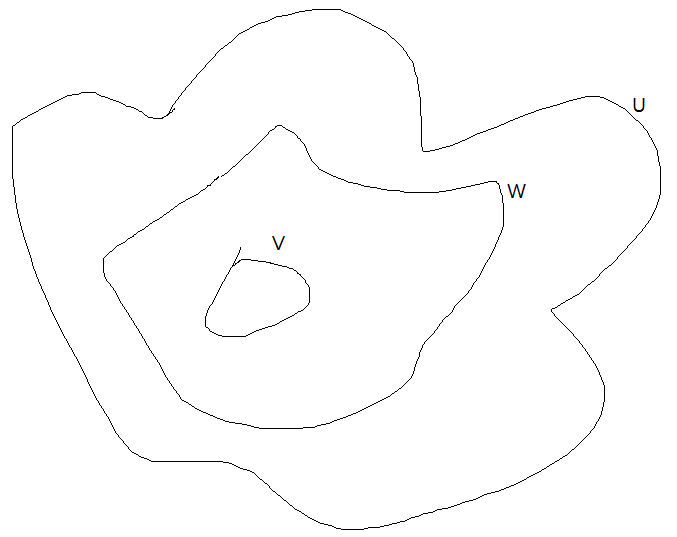
\includegraphics[width=0.5\textwidth]{7}
\end{figure}
\begin{itemize}
\item[1.] Fix $V \subset \subset U$ and choose $W$ such that $V \subset\subset W \subset\subset U$. Take $\zeta \in C_c^{\infty}(W)$ such that $\zeta \equiv 1$ on $V$. Rewriting ($\star$) we have
\begin{align*}
\sum_{i,j=1}^n \int_U a^{ij} u_{x_i} v_{x_j} dx = \int_U \tilde{f} v dx \quad \forall v \in H_0^1 (U)
\end{align*} 
where $\tilde{f} = f-\sum_{i=1}^n b^i u_{x_i} -cu \in L^2(U)$.
\item[2.] Let $|h| >0$ be small, fix $k\in \{1,\cdots, n\}$ and take
\begin{align*}
v = -\Delta_k^{-h} (\zeta^2 \Delta_k^h u)
\end{align*}
and write
\begin{align*}
A = \sum_{i,j=1}^n \int a^{ij} u_{x_i} v_{x_j} dx, \quad B = \int_U \tilde{f} v dx
\end{align*}
so that $A=B$.
\item[3.] Note that if $v$, $w$ have compact support in $U$, then $v,w\in L^2(U)$ for $|h|$ small.
\begin{align*}
\int_U u \Delta^{-h}_k wdx = -\int_U (\Delta_k^h u) w dx \quad \text{(\textbf{Integration by parts})}
\end{align*}
and $\Delta_k^h (vw) = (\tau^h_k v)\Delta_k^h w + w\Delta_k^h v$ where $\tau_k^h v(x) = v(x+he_k)$ \textbf{(Leibniz rule)}. Also, $(\Delta_k^h u)_{x_i} = \Delta_k^h u_{x_i}$ (\textbf{commutation rule}). We estimate $A$ as follows :
\begin{align*}
A &= -\sum_{i,j} \int_U a^{ij} u_{x_i} \Big[ \Delta_k^{-h} (\zeta^2 \Delta_k^h u) \Big]_{x_j} dx \\
&= -\sum_{i,j} \int_U a^{ij} u_{x_i} \Delta_k^{-h} (\zeta^2 \Delta_k^h u)_{x_j} dx \\
&= \sum_{i,j} \int_U \Delta_k^{h}(a^{ij} u_{x_i}) \cdot (\zeta^2 \Delta_k^h u)_{x_j} dx \\
&= \sum_{ij} \int_U (\tau_k^h a^{ij} \Delta_k^h u_{x_i} + \Delta_k^h (a^{ij}) u_{x_i})(\zeta^2 \Delta_k^h u_{x_j} + 2\zeta \zeta_{x_j} \Delta_k^h u) dx
\end{align*}
Expanding, we get
\begin{align*}
A = \sum_{i,j=1}^n \int_U & (\tau_k^h a^{ij}) \Delta_k^h u_{x_i} \Delta_k^h u_{x_j} dx \\
+ \sum_{i,j} \int \Big[ & (\Delta_k^h a^{ij})u_{x_j}\zeta^2 \Delta_k^h u_{x_j} + (\Delta_k^h a^{ij})u_{x_j} \times 2\zeta \zeta_{x_j} \Delta_k^h u \\
& + (\tau_k^h a^{ij})\Delta_k^h u_{x_i} \times 2\zeta \zeta_{x_j} \Delta_k^h u \Big] dx
\end{align*}
Define this to be $A_1 + A_2$. Now, by uniform ellipticity applied to $\tau_k^h a^{ij}$, have
\begin{align*}
A_1 \geq \theta \int_U \zeta^2 |\Delta_k^h Du|^2 dx
\end{align*}
Since $a^{ij}\in C^1(U)$ and $\zeta$ supported in $W$, we have
\begin{align*}
|A_2| \leq C \int_W \zeta |\Delta_k^h Du| |Du| + \zeta |Du||\Delta_k^h u|  + \zeta |\Delta_k^h Du| |\Delta_k^h u| dx
\end{align*}
so by applying Young's inequality(or just AM-GM inequality) twice with an $\epsilon$,
\begin{align*}
|A_2| \leq \epsilon \int_W \zeta^2 |\Delta_k^h Du| dx + \frac{C}{\epsilon} \int_W |Du|^2 + |\Delta_k^h u|^2 dx
\end{align*}
Setting $\epsilon=\theta/2$, we have
\begin{align*}
A \geq \frac{\theta}{2} \int_U \zeta^2 |\Delta^h_k Du| dx - C \int_W |Du|^2 dx
\end{align*}
\end{itemize}
\end{proof}


%졸라 배고파,,,,,,,
\end{document}